%% BioMed_Central_Tex_Template_v1.06
%%                                      %
%  bmc_article.tex            ver: 1.06 %
%                                       %

%%IMPORTANT: do not delete the first line of this template
%%It must be present to enable the BMC Submission system to
%%recognise this template!!


%%% additional documentclass options:
%  [doublespacing]
%  [linenumbers]   - put the line numbers on margins

%%% loading packages, author definitions

%\documentclass[twocolumn]{bmcart}% uncomment this for twocolumn layout and comment line below
\documentclass{bmcart}

%%% Load packages
%\usepackage{amsthm,amsmath}
%\RequirePackage{natbib}
%\RequirePackage[authoryear]{natbib}% uncomment this for author-year bibliography
%\RequirePackage{hyperref}
\usepackage[utf8]{inputenc} %unicode support
\usepackage{algorithmic}
\usepackage{rotating}
\usepackage{amsmath}
\usepackage{multirow}
\usepackage{enumerate}
\usepackage{algorithm}
\usepackage{subfigure}
%\usepackage[applemac]{inputenc} %applemac support if unicode package fails
%\usepackage[latin1]{inputenc} %UNIX support if unicode package fails


%%%%%%%%%%%%%%%%%%%%%%%%%%%%%%%%%%%%%%%%%%%%%%%%%
%%                                             %%
%%  If you wish to display your graphics for   %%
%%  your own use using includegraphic or       %%
%%  includegraphics, then comment out the      %%
%%  following two lines of code.               %%
%%  NB: These line *must* be included when     %%
%%  submitting to BMC.                         %%
%%  All figure files must be submitted as      %%
%%  separate graphics through the BMC          %%
%%  submission process, not included in the    %%
%%  submitted article.                         %%
%%                                             %%
%%%%%%%%%%%%%%%%%%%%%%%%%%%%%%%%%%%%%%%%%%%%%%%%%

%\def\includegraphic{}
%\def\includegraphics{}

%%% Put your definitions there:
\startlocaldefs
\endlocaldefs



\begin{document}
\begin{frontmatter}
\begin{fmbox}
\dochead{Research}

\title{Improving the performance of Bayesian phylogenetic inference under relaxed clock models}

\author[
   %addressref={aff1},                   % id's of addresses, e.g. {aff1,aff2}
   %email={rzha419@aucklanduni.ac.nz}
]{\inits{}\fnm{Rong} \snm{Zhang}}
\author[
   addressref={aff1},
   corref={aff1},                       % id of corresponding address, if any
   email={alexei@cs.auckland.ac.nz}   % email address
   %noteref={n1},                        % id's of article notes, if any
]{\inits{}\fnm{Alexei} \snm{Drummond}}

\address[id=aff1]{%                           % unique id
  \orgname{School of Computer Science, University of Auckland}, % university, etc
  \street{Princes Street},                     %
  \postcode{1010}                                % post or zip code
  \city{Auckland},                              % city
  \cny{New Zealand}                                    % country
}

%\address[id=aff2]{%
%  \orgname{},
%  \street{},
%  \postcode{}
%  \city{},
%  \cny{}
%}

%\begin{artnotes}
%%\note{Sample of title note}     % note to the article
%\note[id=n1]{Equal contributor} % note, connected to author
%\end{artnotes}

\end{fmbox}% comment this for two column layout

%%%%%%%%%%%%%%%%%%%%%%%%%%%%%%%%%%%%%%%%%%%%%%
%%                                          %%
%% The Abstract begins here                 %%
%%                                          %%
%% Please refer to the Instructions for     %%
%% authors on http://www.biomedcentral.com  %%
%% and include the section headings         %%
%% accordingly for your article type.       %%
%%                                          %%
%%%%%%%%%%%%%%%%%%%%%%%%%%%%%%%%%%%%%%%%%%%%%%
\begin{abstractbox}
\begin{abstract}
Bayesian MCMC has become a common approach for phylogenetic inference. This paper develops a new operator to improve the efficiency of Bayesian phylogenetic inference for models that include a per-branch rate parameter. In an MCMC algorithm, the proposed operator changes evolutionary rates and divergence times at the same time, under the constraint that the implied genetic distances remain constant. Specifically, the proposal operates on the divergence time of an internal node and the three adjacent branch rates. For the root of a phylogenetic tree, there are three strategies discussed, named Simple Distance, Small Pulley and Big Pulley. It is noticed that Big Pulley is able to change the tree topology, which enables the operator to sample all the possible rooted trees consistent with the implied unrooted tree. To validate its effectiveness, a series of experiments have been performed by implementing the proposed operator in the BEAST2 software. The results demonstrate that the proposed operator is able to improve the performance by giving better estimates and using less running time. Measured by effective samples per hour, the proposed operator is at least four times faster than the current operators in BEAST2.
\end{abstract}

\begin{keyword}
\kwd{Bayesian MCMC}
\kwd{Operator}
\kwd{Genetic distances}
\kwd{Divergence times}
\kwd{Evolutionary rates}
\end{keyword}

% MSC classifications codes, if any
%\begin{keyword}[class=AMS]
%\kwd[Primary ]{}
%\kwd{}
%\kwd[; secondary ]{}
%\end{keyword}

\end{abstractbox}
%
%\end{fmbox}% uncomment this for twcolumn layout
\end{frontmatter}

%%%%%%%%%%%%%%%%%%%%%%%%%%%%%%%%%%%%%%%%%%%%%%
%%                                          %%
%% The Main Body begins here                %%
%%%%%%%%%%%%%%%%%%%%%%%%%%%%%%%%%%%%%%%%%%%%%%

%%%%%%%%%%%%%%%%
\section*{Introduction}
Bayesian phylogenetics puts an emphasis on estimating probability distributions of parameters of interest, including the phylogenetic tree topology and divergence times, given the data. 
Markov chain Monte Carlo (MCMC) has been the primary computational tool used in Bayesian phylogenetics for sampling from the posterior distribution. 
Early implementations of Bayesian phylogenetic inference assumed a strict molecular clock in order to estimate divergence times \cite{yang1997bayesian,rannala2003bayes}, but the introduction of relaxed molecular clocks allowed for the estimation of divergence times in the presence of rate heterogeneity among branches. 

Bayesian phylogenetic inference via MCMC is computationally intensive for large data sets. 
Two approaches to improve efficiency are (i) improved proposal mechanisms and (ii) faster phylogenetic likelihood calculations.

Calculating the phylogenetic likelihood is computationally expensive. 
Hence, researchers have tried many ways to tackle the computation burden in the likelihood calculations, such as detection of repeating sites \cite{kobert2017efficient},  approximate methods (e.g. \cite{reis2011approximate}) and the use of parallelisation strategies. 

However the overall efficiency of the sampling process also depends strongly on the construction of the proposal mechanism. 
More efficient proposal mechanisms require fewer steps in the MCMC chain and thus fewer likelihood computations, since each step of the MCMC chain entails a likelihood calculation. 

A major limitation in Bayesian MCMC analysis of phylogeny lies in the efficiency with which operators sample the tree space \cite{lakner2008efficiency}. 
%Many such tree proposal mechanisms have been described \cite{}. %According to the work in Ref.\cite{hohna2011guided}, the two common operators, i.e. prune-and-regraft and subtree-swap, both contribute to a tree with low likelihood since they propose a new tree by random movement of the current tree. So the authors introduced two new operators by proposing a state from a discrete set of possible proposals and narrowing the proposal distribution to the more likely proposals. Their experimental results proved that the two operators have faster average run time and more accurate predictability.
Nevertheless, it is acknowledged that faster and more reliable estimation is also dependent on a good mixture of operators in Bayesian MCMC, since the posterior distribution often exhibits correlations between the tree and other random variables. 

In this paper, a novel operator is proposed that moves within a subspace of constant genetic distances. 
Namely, the proposed operator changes both divergence times of nodes and neighbouring branch rates so that implied genetic distances are not changed. 
For time-reversible substitution models the phylogenetic likelihood will also be unchanged under this operation. 
The proposed operator has been implemented and tested in BEAST2 \cite{}. 

%The paper is constructed as follows: Section 2 gives some preliminary theory related to this paper. 
%Section 3 introduces the proposed operator, which includes the operations for internal nodes and three different strategies for the root. 
%The experiments and discussions are detailed in Section 4 to validate the efficiency of the proposed operator. 
%Section 5 ends the paper with a short conclusion.
\section*{Prelimiaries}
\subsection*{Bayesian MCMC}
Equation \ref{bayes} shows a basic Bayesian framework for phylogenetic inference. It consists of prior distributions for the tree $g$ and a set of parameters of interest $\Phi $, a phylogenetic likelihood that conveys information from data $D$, and the posterior distribution to be inferred, which are denoted in the form of probability densities by $p(g) $, $p(\Phi )$, $\Pr(D|g,\Phi )$, $f(g,\Phi |D)$ correspondingly. From a Bayesian perspective, the phylogenetic trees and the parameters are random variables described by a posterior probability distribution given the observed data, $D$. 
%As a result, it is possible to jointly infer evolutionary history of species  by incorporating various source of information such as molecular data and fossil records.
\begin{equation}\label{bayes}
p(g,\Phi |D) = \frac{{\Pr (D|g,\Phi ) \times p (g) \times p (\Phi )}}{{\Pr (D)}}
\end{equation}

However, due to the large state space and the marginal likelihood being difficulty to calculate, Markov Chain Monte Carlo (MCMC) is adopted to get samples from the posterior distribution. Specifically, MCMC algorithms construct a Markov chain whose stationary distribution is the posterior distribution $p(g,\Phi |D)$, in such a way that the computation of the marginal likelihood $p (D)$ is avoided. 
%In this paper, a Metropolis-Hastings algorithm (MH-MCMC) is implemented, which generates a new state given the current state through a proposal density and accepts the new state with a prescribed probability \cite{metropolis1953equation,hastings1970monte}.
\subsection*{Tree proposals}
\label{treeproposals}
We use the term ``operator" to describe an algorithm that can be used to draw a new state $\theta'$ given an existing state $\theta = \{g,\Phi\}$ from a specific proposal kernel, $q(\theta'|\theta)$ and also return the Hastings-Green ratio for the proposed state transition \cite{}. In MH-MCMC, an operator implements the proposal density and provided relevant information to calculate the acceptance probability for the next proposed state. 

Standard na\"{i}ve operators such as the random walk operator propose a new state by adding a random variate to a component of the state \cite{suchard2005stochastic}. 
Similarly, a scale operator multiplies the current state by a scale factor \cite{higuchi1997monte}. They are suitable for working on a single random variable, or a single component of the model, such as a population size. 
Standard operators for the tree topology and divergence times include the subtree slide operator, Wilson-balding and narrow exchange operators \cite{hohna2008clock}. 
%On top of this, there are also some extended operators available to help give the better performance. For instance, the prune-and-regraft operator selects a random subtree and reattaches the subtree at a new random branch \cite{hohna2011guided}. 

What matters for developing an operator in MH-MCMC is that the proposal should be reversible. In other words, the probability that the operator propose a new state from the current state is required to be equal to the probability that the proposed state goes back to current state. To be specific, let ${\pi (x)}$ be the target probability distribution and $p(x, x')$ be the transition kernel in the continuous Markov chain. The reversibility condition requires that ${\pi (x)}{p(x, x')} = {\pi (x')}{p(x', x)}$. And an operator provides a proposal $q(x, x')$ with some probability $\alpha(x, x')$ that the proposal is accepted. Thus, the reversibility condition is rewritten as ${\pi (x)}{q(x, x')}{\alpha(x, x')} = {\pi (x')}{q(x', x)}{\alpha(x', x)}$. 

Considering the subspace $\varphi_1$ on $x$ and subspace $\varphi_2$ on $x'$, it is assumed that there is a symmetric measure on the combined parametric space $\varphi = {\varphi_1} \times {\varphi_2}$, so that ${\pi (x)}{q(x, x')}$ has a density with respect to a single measure on $\varphi$. Then, Green suggested that the reversibility condition should be satisfied by the detailed balance \cite{green1995reversible}, as is represented by Eq.(\ref{balance}). And according to Peskun' proof, it is optimal to take Eq.(\ref{Ratio}) as the acceptance probability to retain the detailed balance \cite{peskun1973optimum}.

\begin{equation}\label{balance}
\int_A {\pi (x) d_x} {\int_B  {q(x, x')}{\alpha(x, x')} d_x}  = \int_B {\pi (x') d_{x'}}{\int_A {q(x', x)}{\alpha(x', x)} d_{x'}}
\end{equation}
, where $A \in {\varphi_1}$ and $B \in  {\varphi_2}$ are two Borel sets. ${q(x, x')}$ denotes the probability that the operator proposes a new state $x'$ given the current state $x$.

\begin{equation}\label{Ratio}
{\alpha_m }(x, x') = \min \left\{ {1,\frac{{\pi (x'){p}(x',x)}}{{\pi (x){p}(x,x')}}} \right\}
\end{equation}
%, where ${p(x',dx)}/{p(x,dx')}$ is called Hastings ratio

However, for operators that do not have a symmetric measure, it is necessary to include the Jacobian matrix ${\mathbf{J}}$  in order to deal with the dimension matching problem, as is discussed in Green's paper \cite{green1995reversible}. In this case, Eq.(\ref{Ratio}) is extended and defined as Green ratio, shown in Eq.(\ref{Green})
\begin{equation}\label{Green}
{\alpha_G}(x, x') = \min \left\{ {1,\frac{{\pi (x'){p}(x',x)}}{{\pi (x){p}(x,x')}}}\left|{\mathbf{J}}\right| \right\}
\end{equation}
, where ${\mathbf{J}} = {\nabla h(x, x')}$ represents a vector differential matrix of deterministic function $h$ that makes the proposal have a symmetric measure on each subspace in state $x$ and $x'$.

\subsection*{Uncorrelated relaxed clock model}
This paper is aimed at improving the performance of relaxed clock model in Bayesian phylogenetic analysis. First of all, a molecular clock model is used to model how nucleotides evolve with certain rates along branches in the phylogenetic tree, so that a time tree can reconcile with the genetic distances between sequences. In the very beginning, a strict clock model assumes evolutionary rates to be the same at every branch \cite{zuckerkandl1965evolutionary}. But recently, the idea of relaxing the molecular clock has become a research of interest and has been widely applied, such as the study of Nothofagus \cite{knapp2005relaxed}. By allowing rates to vary across lineages, it is considered that better estimates of divergence times can be obtained, according to the work in Ref.\cite{ho2005accuracy,renner2005relaxed,lepage2007general}. 
%%define genetic distance

 In this paper, the proposed operator is based on an uncorrelated relaxed model, where the rates vary and follow a certain distribution. As is detailed in Ref.\cite{drummond2006relaxed}, uncorrelated rates indicate that the rates on branches are identically distributed and will be independently drawn from a certain distribution such as a log-normal distribution. As a result, the rates can change faster than making a slight move over multiple adjoining branches. In 2010, Smith et al. applied an uncorrelated relaxed-clock to flowering plants and the results show the consistency with the fossil record \cite{smith2010uncorrelated}.

Referring to the Bayesian framework shown by Eq.(\ref{bayes}), the joint inference of evolutionary rates and divergence times can be obtained by the conditional distribution in Eq.(\ref{bayes1}). And the proposed operator is to sample the state $(t,r,\Phi)$ in the constructed Markov chain.
\begin{equation}\label{bayes1}
p(t,r,\Phi |D) = \frac{{p(D|t,r,\Phi )p(r|\Phi )p(t|\Phi )p(\Phi )}}{{p(D)}}
\end{equation}
, where $p(r|\Phi )$ is the prior for rates specified in uncorrelated relaxed clock model.
\section*{Methodology: the proposed operator}
In this section, we define the proposed operator as ConstantDistance Operator. Fig.\ref{flowchart} illustrates the flow chart of the proposed operator. In a phylogenetic tree, the node to operate on is denoted by \textbf{X}. The proposed operator works differently on the internal nodes and the root of the tree. The details of the operations are introduced step by step in the following subsections.
\subsection*{Operations on internal nodes}
Fig.\ref{internalnodes} represents the tree (or subtree of a phylogenetic tree) with the node \textbf{X} that is randomly selected among the internal nodes. The original tree in the current state is denoted by $g_{in}$. And the following 5 steps will propose a new tree ${g_{in}}'$.

\emph{Step 1} Get the parent node and two child nodes of \textbf{X}, denoted by \textbf{P}, \textbf{L} and \textbf{R} respectively.

\emph{Step 2} Get the nodes times of \textbf{X}, \textbf{P}, \textbf{L} and \textbf{R} , denoted by $t_X$, $t_P$, $t_1$, $t_2$, as well as the rates on the branches above the nodes, denoted by $r_i$, $r_j$, $r_k$.

\emph{Step 3} Propose a new node time for \textbf{X} by ${t_X}' = {t_X} + a$, where $a$ follows a Uniform distribution with a symmetric window size, i.e. $a \sim U[ - w, + w]$. Make sure that the proposed time is valid, i.e. $\max \{ {t_1},{t_2}\}  < {t_X}' < {t_P}$ holds.

\emph{Step 4} Propose new rates by using Eq.(\ref{int_rate}).
\begin{equation}
 \label{int_rate}
{r_i}' = \frac{{r_i} \times ({{t_P} - {t_X}})}{{{t_P} - {t_X}'}}\\
{r_j}' = \frac{{{r_j} \times ({{t_X} - {t_1}})}}{{{t_X}' - {t_1}}}\\
{r_k}' = \frac{{{r_k} \times ({{t_X} - {t_2}})}}{{{t_X}' - {t_2}}}
 \end{equation}

\emph{Step 5} Return the Hastings ratio.
\subsection*{Operations on the root}
For the root of the tree, there are three strategies to propose the new rates and node times. To be more specific, Simple Distance is a way of proposing a new root time only. Considering the genetic distance, Small Pulley adjusts the distances of branches on both sides of the root. Moreover, under the constraint that the unrooted tree is fixed, Big Pulley proposes a new tree topology by rearranging the root.  Details are discussed below
\subsubsection*{Simple Distance}
Fig.\ref{simpledistance} shows the trees that are rooted at the node $X$. The original tree in the current state is shown in Fig.\ref{simpledistance}(a), which is denoted by $g_r$. Inspired by the operations on internal nodes, we will use the following steps to propose a new tree ${g_{r1}}'$, and keep the genetic distances $d_i$ and $d_x$ constant at the same time. The steps are illustrated in Fig.\ref{simpledistance}(b).

\emph{Step 1} Get the child nodes of the root \textbf{X}, denoted by \textbf{L} and \textbf{R}. Their corresponding node times and rates are $t_X$, $t_j$, $t_k$ and $r_i$, $r_x$.

\emph{Step 2} Propose a new node time for the root \textbf{X} by \textbf{X} by ${t_X}' = {t_X} + a$, where $a \sim U[ - w, + w]$. Make sure that ${t_X}' > \max \{ {t_j},{t_k}\} $ holds.

\emph{Step 3} Propose new rates for branches on both sides of the root by using Eq.(\ref{sim_rate}).
\begin{equation}
\label{sim_rate}
{r_i}' = \frac{{{r_i} \times ({{t_X} - {t_j}})}}{{{t_X}' - {t_j}}}\\
{r_x}' = \frac{{{r_x} \times ({{t_X} - {t_k}})}}{{{t_X}' - {t_k}}}
 \end{equation}

\emph{Step 4} Return the Hastings ratio.
\subsubsection*{Small Pulley}
Different from Simple Distance, a new genetic distance of branch on one side of the root is proposed in Small Pulley. As is illustrated in Fig.\ref{simpledistance}, Small Pulley proposes a new tree ${g_{r2}}'$ in Fig.\ref{simpledistance}(c), based on the original tree $g_r$ in Fig.\ref{simpledistance}(a). In order to maintain the total genetic distance of $d_i$ and $d_x$, once ${d_i}'$ is proposed, $d_x$ will be adjusted simultaneously. The detailed process includes the following 4 steps.

\emph{Step 1} Get the child nodes of the root \textbf{X}, denoted by \textbf{L} and \textbf{R}. Their corresponding node times and rates are $t_X$, $t_j$, $t_k$ and $r_i$, $r_x$. So the genetic distances of the two branches linked to the root can be calculated according to Eq.(\ref{sma1_dis}).
\begin{equation}
\label{sma1_dis}
{d_i} = {r_i} \times ({{t_X} - {t_j}})\\
{d_x} = {r_x} \times ({{t_X} - {t_k}})
 \end{equation}

\emph{Step 2} Propose a new genetic distance for $d_i$ by adding a random number that follows a Uniform distribution, i.e.  ${d_i}' = {d_i} + b$, where $b \sim U[ - v, + v]$. Make sure that $0 < {d_i}' < D$ holds, where $D = {d_i} + {d_x}$.

\emph{Step 3} Propose new rates for branches on each side of the root by using Eq.(\ref{sma1_rate}).
\begin{equation}
\label{sma1_rate}
{r_i}' = \frac{{{d_i}'}}{{{t_X} - {t_j}}}\\
{r_x}' = \frac{{D - {d_i}'}}{{{t_X} - {t_k}}}
 \end{equation}

\emph{Step 4} Return the Hastings ratio.
\subsubsection*{Big Pulley}
Big Pulley is used to sample the rates and times from a fixed unrooted tree, in the meantime, the genetic distances among taxon are constant, which means the location of the root will be rearranged.

Firstly, a method called \textit{Exchange (,)} is designed to propose a new tree topology in this circumstances. To be specific, for the original tree $g$ in Fig.\ref{exchangemethod}, once the method \textit{Exchange (\textbf{M},\textbf{N})} is called, the following operations will be performed to proposed a new tree $g'$.
\begin{itemize}
\item Exchange \textbf{M} and \textbf{N} by pruning and grafting, i.e. cutting \textbf{M} (\textbf{N}) at its original position and attaching it to the original position of \textbf{N} (\textbf{M}).
\item Propose ${d_C}'$ by ${d_C}' = {d_C} + b$, where $b \sim U[ - v, + v]$. Make sure that $0 < {d_C}' < D$ holds, where $D = {d_C} + {d_{N}}$.
\item The distances on the other three branches, i.e. $d_S$, $d_{M}$ and $d_{N}$, will be adjusted by using Eq.(\ref{big_dis}).
\begin{equation}\label{big_dis}
{d_S}' = {d_S}\\
{d_{M}}' = {d_{M}} - {d_C}'\\
{d_{N}}' = {d_{N}} + {d_C}
\end{equation}
\end{itemize}

As can be seen from the above descriptions, the method \textit{Exchange (\textbf{M},\textbf{N})} is actually aimed at swapping two nodes and reassigning distances on the four branches. That is to say, after using \textit{Exchange (\textbf{M},\textbf{N})}, the distances $d_S$, $d_{M}$, $d_{N}$ and $d_{C}$ will be adjusted to maintain the distances among three taxa \textbf{S}, \textbf{M} and \textbf{N}, as the tree topology changes. 

Secondly, before applying this method in Big Pulley, there are two different tree shapes to take into consideration. In Fig.\ref{treeshape}, a symmetric tree is shown on the left, in which both the child nodes of the root have child nodes. But in the asymmetric tree on the right, only one of the child nodes of the root has child nodes below it, which means the other child node of the root is a leaf node. Hence, Big Pulley also differs when it works on a symmetric and asymmetric tree. The corresponding operations are detailed in the following two parts.
\paragraph*{Symmetric tree shape}

For the symmetric tree in Fig.\ref{treeshape}, the operations are illustrated in Fig.\ref{symmetric}, after which one of the four possible trees (\textcircled1 \textcircled2 \textcircled3 \textcircled4) will be proposed.

\emph{Step 1} Get the child nodes of the root \textbf{X}, denoted by \textbf{L} and \textbf{R}. Correspondingly, the node times are denoted by $t_X$, $t_j$, $t_k$. And the child nodes below them are denoted by $H1$, $H2$, $H3$ and $H4$. 

\emph{Step 2} Propose a new node time for the root \textbf{X} by ${t_X}' = {t_X} + a$, where $a \sim U[ - w, + w]$.

\emph{Step 3} Propose a new node time either for \textbf{L} or \textbf{R}. And apply the method using \textbf{R} and either child node of \textbf{L}.
\begin{itemize}
\item With 0.5 probability to pick \textbf{L} and propose a new node time by ${t_j}' = {t_j} + {a_1}$, where ${a_1} \sim U[ - w, + w]$. Make sure that ${t_k} < {t_j}' < {t_X}'$ holds. Then, there are two options to apply the method, i.e.

\textcircled1: With 0.5 probability to apply \textit{Exchange (\textbf{H1} and \textbf{R})}

\textcircled2: With 0.5 probability to apply \textit{Exchange (\textbf{H2} and \textbf{R})}

\item With 0.5 probability to pick \textbf{R} and propose a new node time by ${t_k}' = {t_k} + {a_2}$, where ${a_2} \sim Uniform[ - w, + w]$. Make sure that ${t_j} < {t_k}' < {t_X}'$ holds. Similarly, there are two options to apply the method, i.e.

\textcircled3: With 0.5 probability to apply \textit{Exchange (\textbf{H3} and \textbf{L})}

\textcircled4: With 0.5 probability to apply \textit{Exchange (\textbf{H4} and \textbf{L})}
\end{itemize}

\emph{Step 4}  Update the rates using the adjusted genetic distances divided by the proposed node times. For example, suppose we are going to propose tree \textcircled1. After the new node times for the root \textbf{X} and \textbf{L} are proposed, we apply the method by \textit{Exchange (\textbf{H1} and \textbf{R})}, so that four distances are adjusted, as is shown in Eq.(\ref{example1.1}). Finally, the new rates are updated by using Eq.(\ref{example1.2}).
\begin{equation}\label{example1.1}
{d_1}' = {d_1} - {d_3}'  \\
{d_2}' = {d_2} \\
{d_3}' = {d_3} + b \\
{d_4}' = {d_3} + {d_4}
\end{equation}
\begin{equation}\label{example1.2}
{r_1}' = \frac{{{d_1}'}}{{{t_X}' - {t_1}}} \\
{r_2}' = \frac{{{d_2}'}}{{{t_j}' - {t_2}}} \\
{r_3}' = \frac{{{d_3}'}}{{{t_X}' - {t_j}}} \\
{r_4}' = \frac{{{d_4}'}}{{{t_j}' - {t_k}}} 
\end{equation}
\emph{Step 5} Return the Hastings ratio.
\paragraph*{Asymmetric tree shape}

How to operate on the asymmetric tree in Fig.\ref{treeshape} is illustrated Fig.\ref{asymmetric}, in which there are three possible trees (\textcircled5 \textcircled6 \textcircled7).

\emph{Step 1} Get the older child of the root \textbf{X}, denoted by \textbf{O}, and the younger child of the root is denoted by \textbf{Y}. The node times of the root \textbf{X},  \textbf{O} and its child nodes are denoted by ${t_X}$, ${t_O}$, ${t_{G1}}$ and ${t_{G2}}$ respectively. 

\emph{Step 2} Propose a new node time for the root \textbf{X} by ${t_X}' = {t_X} + a$, where $a \sim U[ - w, + w]$. Moreover, propose a new node time for \textbf{O} by ${t_O}' = {t_O} + {a_3}$, where ${a_3} \sim U[ - w, + w]$. To make it valid, make sure that ${t_O}' < {t_X}'$ holds.  

\emph{Step 3} Apply the method using \textbf{Y} and either child node of \textbf{O}, which is dependent on the value of ${t_O}'$.
\begin{itemize}
\item if ${t_O}'$ satisfies ${t_O}' > \max \{ {t_{G1}},{t_{G2}}\} $ or ${t_{G1}} = {t_{G2}}$, then there are two options, i.e.

\textcircled5: With 0.5 Probability to apply \textit{Exchange (\textbf{G1} and \textbf{Y})}

\textcircled6: With 0.5 Probability to apply \textit{Exchange (\textbf{G2} and \textbf{Y})}
\item if ${t_O}'$ satisfies $\min \{ {t_{G1}},{t_{G2}}\}  < {t_O}' < \max \{ {t_{G1}},{t_{G2}}\} $, then there is only one option, i.e.

\textcircled7: Exchange the older child of \textbf{O} and \textbf{Y}.  In the example here, we apply \textit{Exchange (\textbf{G1}  and \textbf{Y})}.
\end{itemize}

\emph{Step 4}  Update the rates using the adjusted genetic distances divided by the proposed node times. To give an example, assume we are going to propose tree \textcircled5. Firstly, ${t_X}'$ and ${t_O}'$ are proposed in \emph{Step 3}.  Then, in \emph{Step 4}, the method \textit{Exchange (\textbf{G1} and \textbf{Y})} is applied, after which the four distances are adjusted by Eq.(\ref{example2.1}). As a result, Eq.(\ref{example2.2}) is used to update the four rates.
\begin{equation}\label{example2.1}
{d_{G1}}' = {d_{G1}} - {d_O}'  \\
{d_{G2}}' = {d_{G2}}  \\
{d_O}' = {d_O} + b  \\
{d_Y}' = {d_Y} + {d_O} 
\end{equation}
\begin{equation}\label{example2.2}
{r_{G1}}' = \frac{{{d_{G1}}'}}{{{t_X}' - {t_{G1}}}} \\
{r_{G2}}' = \frac{{{d_{G2}}'}}{{{t_O}' - {t_{G2}}}} \\
{r_O}' = \frac{{{d_O}'}}{{{t_X}' - {t_O}}} \\
{r_Y}' = \frac{{{d_Y}'}}{{{t_O}' - {t_Y}}} 
\end{equation}
\emph{Step 5} Return the Hastings ratio.

\subsection*{Calculate the Hastings ratio}
As is mentioned in the previous section, the operator in phylogenetic analysis based on Bayesian MCMC should make a reversible proposal to satisfy the detailed balance (Eq.(\ref{balance})). Therefore, the last step of all the operations in the ConstantDistance Operator is to calculate the Hastings ratio for the acceptance probability (Eq.(\ref{Ratio})). 

According to the third and forth steps in the operations for internal nodes, three rates on the branches linked to the selected internal node are proposed by one random number $a$ that is used to change the node time. There are four parameters involved in this proposal, including 3-dimensional rate space and 1-dimensional time space. The proposed operator utilises one random number in time space and makes changes in both time space and rate space, which leads to the inconsistency in parametric spaces. To solve this dimension-matching problem, as is mentioned in Green's paper \cite{green1995reversible}, it is necessary to construct a Jacobian matrix.  In Eq.(\ref{JacobianMatrix}), ${\mathbf{J_1}}$ deals with the parametric spaces before the proposal in vector ${\mathbf{X}} = [{t_X},{r_i},{r_j},{r_k}]$ and after the proposal in vector ${\mathbf{Y}} = [{t_X}',{r_i}',{r_j}',{r_k}']$.
\begin{equation}\label{JacobianMatrix}
{\mathbf{J_1}} = \left[ {\begin{array}{*{20}{c}}
  {\frac{{\partial {\mathbf{f}}}}{{\partial {t_x}}}}&{\frac{{\partial {\mathbf{f}}}}{{\partial {r_i}}}}&{\frac{{\partial {\mathbf{f}}}}{{\partial {r_j}}}}&{\frac{{\partial {\mathbf{f}}}}{{\partial {r_k}}}}
\end{array}} \right] = \left[ {\begin{array}{*{20}{c}}
  {\frac{{\partial {f_1}}}{{\partial {t_X}}}}&{\frac{{\partial {f_1}}}{{\partial {r_i}}}}&{\frac{{\partial {f_1}}}{{\partial {r_j}}}}&{\frac{{\partial {f_1}}}{{\partial {r_k}}}} \\
  {\frac{{\partial {f_2}}}{{\partial {t_X}}}}&{\frac{{\partial {f_2}}}{{\partial {r_i}}}}&{\frac{{\partial {f_2}}}{{\partial {r_j}}}}&{\frac{{\partial {f_2}}}{{\partial {r_k}}}} \\
  {\frac{{\partial {f_3}}}{{\partial {t_X}}}}&{\frac{{\partial {f_3}}}{{\partial {r_i}}}}&{\frac{{\partial {f_3}}}{{\partial {r_j}}}}&{\frac{{\partial {f_3}}}{{\partial {r_k}}}} \\
  {\frac{{\partial {f_4}}}{{\partial {t_X}}}}&{\frac{{\partial {f_4}}}{{\partial {r_i}}}}&{\frac{{\partial {f_4}}}{{\partial {r_j}}}}&{\frac{{\partial {f_4}}}{{\partial {r_k}}}}
\end{array}} \right]
\end{equation}
, where the functions ${f_1}$, ${f_2}$, ${f_3}$ and ${f_4}$ represent how the operator makes an proposal, i.e. the way of proposing new values. After substituting Eq.(\ref{int_rate}) in Eq.(\ref{JacobianMatrix}), the Hastings ratio for the internal nodes can be derived by Eq.(\ref{HR1}).
\begin{equation}\label{HR1}
{r_1} = \frac{{p ( - a)}}{{p (a)}}\left| {\mathbf{J_1}} \right| = \frac{{{t_P} - {t_X}}}{{{t_P} - {t_X}'}} \times \frac{{{t_X} - {t_1}}}{{{t_X}' - {t_1}}} \times \frac{{{t_X} - {t_2}}}{{{t_X}' - {t_2}}}
\end{equation}
, where the probability ${\Pr ( - a)}$ is equal to ${\Pr ( a )}$ since the random number $a$ is drawn from a Uniform distribution.

Likewise, the Hastings ratio for Simple Distance and Small Pulley can be obtained by Eq.(\ref{HR2}) and Eq.(\ref{HR3}) correspondingly. For the strategy of Big Pulley, the operations are concerned with tree topology. Firstly, to make the proposed topology reversible, a factor $\mu$ is defined and will be included in the Hastings ratio, which is calculated by Algorithm \ref{alg1}. Then, after specifying the Jacobian matrix, the Hastings ratio for Big Pulley is derived by Eq.(\ref{HR4}). More details of the determinant of Jacobian matrix are explained in the Appendix. 
\begin{equation}\label{HR2}
{r_2} = \frac{{p( - a)}}{{p(a)}}\left| {{{\mathbf{J}}_2}} \right| = \frac{{{t_X} - {t_j}}}{{{t_X}' - {t_j}}} \times \frac{{{t_X} - {t_k}}}{{{t_X}' - {t_k}}}
\end{equation}
\begin{equation}\label{HR3}
{r_3} = \frac{{p( - b)}}{{p(b)}}\left| {{{\mathbf{J}}_3}} \right| = 1
\end{equation}
\begin{equation}\label{HR4}
{r_4} = \frac{{p( - a)}}{{p(a)}}\frac{{p( - {a_x} )}}{{p({a_x} )}}\mu \left| {{{\mathbf{J}}_4}} \right| = \frac{{{t_X}' - {t_C}}}{{{t_X}' - {t_C}'}} \times \frac{{{t_C} - {t_S}}}{{{t_C}' - {t_S}}} \times \frac{{{t_C} - {t_{N1}}}}{{{t_X}' - {t_{N1}}}} \times \frac{{{t_X} - {t_{N2}}}}{{{t_C}' - {t_{N2}}}}
\end{equation}
\section*{Experimental results and analysis}
In this section, a series of experiments are conducted by implementing the proposed operator in BEAST2. Some analysis are also included to validate the effectiveness and efficiency of the proposed operator. Firstly, by sampling from the prior distributions, in which no alignments are involved, the correctness of the operator is proved. After the well-calibrated simulation study, it turns out that the operator is able to work properly with other operators and sample the simulated data with reliability. Besides, by comparing ESS and running time, it is demonstrated that the performance is improved when using the proposed operator. Finally, the correlation of rates and node times is discussed, and some potential problems are mentioned in the future work. 
\subsection*{Sample from the prior}
In Fig.\ref{sampleprior}, a tree with three taxa $A$, $B$ and $C$ is used as a small example in this experiment. In the figure, $g_1$ is set as the initial tree. Firstly, a LogNormal distribution is used as the rate prior in the uncorrelated relaxed clock model, given by Eq.(\ref{rateprior}).
\begin{equation}\label{rateprior}
r = [{r_i}\quad{r_j}\quad{r_k}\quad{r_x}] \sim LogNormal(M = -3, S = 0.5)
\end{equation}

In addition, a Coalescent model with constant population size ($N=0.3$) is used to describe the tree prior. Hence, for the tree in Fig.\ref{sampleprior}, the probability of node times is calculated by Eq.(\ref{treeprior}).
\begin{equation}\label{treeprior}
p({t_E},{t_D}) = (\frac{1}{N} \times {e^{ - \frac{1}{N}({t_E} - {t_D})}}) \times (\frac{1}{N} \times {e^{ - \frac{3}{N}{t_D}}})
\end{equation}

After the priors are specified, the distribution to sample can be exactly known, since the samples are drawn from the prior distributions. In other words, as the rates are functions of its genetic distance and times, the joint distribution to sample can be represented by Eq.(\ref{integration}).
\begin{equation}\label{integration}
\begin{aligned}
p(r,t) &= p({t_E},{t_D}) \times p({r_i}) \times p({r_j}) \times p({r_k}) \times p({r_x}) \\&= P({t_E},{t_D}) \times p(\frac{{{d_i}}}{{\Delta t1}}) \times p(\frac{{{d_j}}}{{\Delta t2}}) \times p(\frac{{{d_k}}}{{\Delta t3}}) \times p(\frac{{{d_x}}}{{\Delta t4}})
\end{aligned}
\end{equation}
, where ${\Delta t1}$, ${\Delta t2}$, ${\Delta t3}$, ${\Delta t4}$ represents the time duration along the corresponding branch, and $p({.})$ is the probability of certain rate values in the LogNormal distribution. Therefore, the whole probability can be obtained by conducting numerical integration on Eq.(\ref{integration}), which shows the probability distribution over all the possible values of parameters.
\subsubsection*{Test the operator on internal nodes}
The genetic distances, node times and rates for $g_1$ in Fig.\ref{sampleprior} are given in Table \ref{ini_inter}. To test roundly, two scenarios are designed. In each scenario, the genetic distances are fixed, the node time $t_D$ starts from the initial value and will be changed by the proposed operator during the sampling process. Essentially, the proposed operator makes node $D$ move between node $A$ and $E$. Besides, to make sure that the result is robust, two different MCMC chain lengths are performed in each scenario, i.e. 10 million and 20 million.

The mean, mean error and the standard deviation of the MCMC samples are summarised in Table \ref{res_inter}. Besides, according to Eq.(\ref{integration}), the actual joint distribution is obtained by using Eq.(\ref{integration1}), and is used to evaluate the results, which is also included in Table \ref{res_inter}. Moreover, the histograms of MCMC samples that indicate the sampled distributions, as well as the curves of the numerical integration of Eq.(\ref{integration1}), are shown in Fig.\ref{res_int}. From Table \ref{res_inter} and Fig.\ref{res_int}, it can be seen that the red curves well fit the black histograms, and the mean values and standard deviations are consistent, which makes it safe to conclude that the proposed operator samples the internal node correctly.
\begin{equation}
\label{integration1}
P(r,{t_D}) = \int_{{t_D} = 0}^{{t_E}} {P({t_E},{t_D}) \times P(\frac{{{d_j}}}{{{t_D}}}) \times P(\frac{{{d_k}}}{{{t_D}}}) \times P(\frac{{{d_i}}}{{{t_E} - {t_D}}}) \times P(\frac{{{d_x}}}{{{t_E}}}){d_{t_D}}}
\end{equation}
\subsubsection*{Test the operator on root}
Still starting from $g_1$ in Fig.\ref{sampleprior}, the initial settings for testing the root are given in Table \ref{ini_sim}. And the three strategies are tested separately in the following parts.

\paragraph*{Using Simple Distance}

The root time $t_E$ is sampled by Simple Distance, which ranges from 1 to positive infinity theoretically. Namely, all the genetic distances and the node time $t_D$  are fixed. Similar to Eq.(\ref{integration1}), the joint distribution of $t_E$ and rates to sample can be obtained by Eq.(\ref{integration2}).
\begin{equation}
\label{integration2}
P(r,{t_E}) = \int_{{t_E} = 1}^{ + \infty } {P({t_E},{t_D}) \times P(\frac{{{d_j}}}{{{t_D}}}) \times P(\frac{{{d_k}}}{{{t_D}}}) \times P(\frac{{{d_i}}}{{{t_E} - {t_D}}}) \times P(\frac{{{d_x}}}{{{t_E}}}){d_{t_E}}}
\end{equation}

The results are given in Table \ref{res_sma} and Fig.\ref{Fig.sub.5}. As can be seen, the mean and the standard deviation are close enough, which confirms that the two distribution are the same. Thus, Simple Distance is proved to be correct.

\paragraph*{Using Small Pulley}

Although both ${d_x}$ and ${d_i}$ are changed during the sampling process when using Small Pulley, the sum of ${d_x}$ and ${d_i}$ are kept 0.67 in this test, as the initial setting shown in Table \ref{ini_sim}. To make it simple, only ${d_i}$ is compared.

Then, based on Eq.(\ref{integration}), the exact distribution of ${d_i}$ can be obtained by Eq.(\ref{integration3}), which is compared with the sampled distribution in Table \ref{res_sma} and Fig.\ref{Fig.sub.6}. Even though there exist some errors, the sampled parameters can be considered to follow the same distribution. So the Small Pulley is also able to provide correct samples.
\begin{equation}\label{integration3}
P(r,{d_i}) = \int_{{d_i} = 1}^{0.67} {P({t_E},{t_D}) \times P(\frac{{{d_j}}}{{{t_D}}}) \times P(\frac{{{d_k}}}{{{t_D}}}) \times P(\frac{{{d_i}}}{{{t_E} - {t_D}}}) \times P(\frac{{0.67 - {d_i}}}{{{t_E}}}){d_{d_i}}}
\end{equation}

\paragraph*{Using Big Pulley}

For $g_1$ in Fig.\ref{sampleprior} with tree taxa, a new tree, together with the root time $t_E$ and node time of its older child $t_D$, as well as a genetic distance $d_i$, is proposed by Big Pulley. In this case, the initial tree $g_1$ will either go to $g_2$ or $g_3$, as is shown in Fig.\ref{sampleprior}.  So the samples are repeatedly drawn from the 3 trees. Besides, according to the initial settings in Table \ref{ini_sim}, the genetic distances remain unchanged during the process, i.e. $d_{AB} = 1$, $d_{AC}  = 1$ and $d_{BC} = 1$ hold. Hence, the distribution we are about to achieve can be calculated by Eq.(\ref{integration5}).
\begin{equation}\label{integration5}
\begin{aligned}
P({t_E},{t_D},{d_i}) &= \int_{{t_E} = 0}^{ + \infty } {\int_{{t_D} = 0}^{{t_E}} {\int_{{d_i} = 0}^{0.5} {P({t_E},{t_D})} } \times P(\frac{{0.5}}{{{t_D}}})}  \\&\times P(\frac{{0.5}}{{{t_D}}}) \times P(\frac{{{d_i}}}{{{t_E} - {t_D}}}) \times P(\frac{{0.5 - {d_i}}}{{{t_E}}}){d_{d_i}}{d_{t_D}}{d_{t_E}}
\end{aligned}
\end{equation}

The statistical measurements, i.e. mean and standard deviation, are compared in Table \ref{res_sma}. The histograms of samples and theoretical distributions of ${d_i}$ and ${t_E}$ are pictured in Fig.\ref{Fig.sub.9} and Fig.\ref{Fig.sub.10}. It is shown that the two distributions are consistent within the acceptable error range. Therefore, Big Pulley can also give the right combinations of rates and node times, under the condition that the genetic distances among taxa are constant.


\subsection*{Well-calibrated simulation study}
As is discussed in Ref.\cite{dawid1982well}, a well-calibrated simulation study is a necessary criterion to evaluate the reliability of probability forecasting. Hence, this section is to verify how reliable the predictions are in the phylogenetic analysis using the proposed operator.

Fig.\ref{modelvalidation} shows the framework used in this study, including the genetic models and prior distributions of parameters. As is shown in the figure, the sequence alignment is simulated by a phylogenetic continuous-time Markov chain in BEAST2. In the Markov chain, it contains a mutation rate matrix given by HKY model and a substitution tree jointly provided by uncorrelated relaxed clock model and Yule model. More specifically, base frequencies $\pi = (\pi_{A}, \pi_{C}, \pi_{T}, \pi_{G})$ follow a Dirichlet distribution and the ratio of transition and transversion rate $\kappa$ follows a LogNormal distribution. The distribution of node times is described in a Yule tree $\Psi$ with birth rate $\lambda $ following a LogNormal distribution. The rates on branches $r_i$ have a LogNormal distribution with mean equaling to 1 and the standard deviation $S1$ following a hyper prior distribution.  

In the first place, 100 independent samples of each parameter are obtained from their prior distributions, including UcldStdev $S1$, BirthRate $\lambda $, Frequency $\pi$ and Kappa $\kappa$. Then, the samples are utilised to simulate nucleotide sequences. To make this study more robust, two groups of sequence data are simulated, one group with 20 taxa and the other with 120 taxa ($n=2/120$). So there are 100 sets of sequence alignment in each group and all the sequences have same length (10 thousand site). 

In the second place, the 200 simulated data sets from two groups are specified in 200 seperate XML files. And all the XML files include the ConstantDistance Operator as well as the same models in Fig.\ref{modelvalidation}.  Afterwards, the XML files are run by BEAST2 software. 

Finally, the estimated values of the parameters are compared with the real values that are used to simulate the sequence alignment. The comparisons of the two groups are shown in Fig.\ref{SmallTree} and Fig.\ref{LargeTree}. It is noticed in the figure that 95\% HPD of the mean values of sampled rates are compared with 1, because the mean rate is fixed during the analysis. Besides, the height of the tree, which is determined by birth rate in Yule model, is considered as a random variable and is also compared in the figure. As is indicated in the figure, most real values of the parameters are within the 95\% HPD of the sampled distribution. According to Table \ref{num_hpd}, on average, 95 percent of estimated values are close to their corresponding real values. Therefore, it is proved that the proposed operator is able to provide reliable estimations for both small ($n=20$) and large ($n=120$) data sets.
\subsection*{Performance comparison}
For Bayesian phylogenetic analysis based on BEAST2, the performance is concerned with how well the parameters are estimated and how much time it requires to run an MCMC chain. Effective Sample Size (ESS) of a parameter is the number of effectively independent draws from the posterior distribution. The larger ESS indicates the better estimation of the parameter.  Besides, whether the ConstantDistance Operator is time-consuming or not is quantified by the time for BEAST2 to finish running the input XML file. Therefore, ESS and running time are adopted to valuate the performance of the ConstantDistance Operator. 

In addition, to make comparisons, the exact same data set will be specified in XML files. The genetic models and prior distributions are also the same in all XML files. But the configurations of operators are different in the aspects of 1) using current operators in BEAST2 to sample discrete rate categories (categories), 2) using the ConstantDistance Operator  to sample continuous rates specified in uncorrelated relaxed clock model(cons), and 3) without using the ConstantDistance Operator to sample continuous rates (nocons). Moreover, because of the randomness of an MCMC chain, each XML file will be run 100 times. Last but not Least, all the running jobs are submitted to Mahuika, a platform of NeSI that provides high performance computing \cite{nesi}.  After running the XML files by using one CPU and one single thread, the user time of each job is recorded as the running time of the corresponding simulation. And ESS of the parameters are obtained by Tracer V.16, a programme for analysing log files output by softwares such as BEAST2 \cite{Tracer}.

\subsubsection*{Analysis of a simulated data set}
The same framework in Fig.\ref{modelvalidation} is used to simulate two groups of sequence alignment. The first group has 20 taxa and the second group has 120 taxa. In each group, there are three data sets with different sequence length. Hence, there are six data sets in total, i.e. two sets of  sequences with 20 thousand sites (long), two sets of  sequences with 10 thousand sites (medium) and two sets of sequences with 5 thousand sites (short). Each data set is firstly specified in three XML files using configurations detailed above, and then will be run 100 times in BEAST2. 

The ESS and running time are summarised in Fig.\ref{eff_comp} and Table \ref{eff_comp1}. According to the two pictures at the top of Fig.\ref{eff_comp}, for different sequence lengths in the two groups with 20 and 120 taxon, most results of 100 analysis show that the configuration using the proposed operator achieves much larger ESS, compared with ESS in other two configurations. Besides, as is indicated in the two pictures at the bottom of Fig.\ref{eff_comp}, the running time is decreased to some degree, in most cases where the proposed operator is used. And this trend is more obvious for a large data set. Table \ref{eff_comp1} lists the mean values of ESS and running time for the 100 analysis of each data set, based on which the value of ESS achieved in an hour (ESS per hour) is also calculated. It implies that the configuration using the proposed operator achieves 4.02 and 4.23 times larger ESS per hour, for 20 taxa and 120 taxa respectively, compared with configuration without using the proposed operator (nocons). And the improvement is more obvious when it is compared with configuration using rate categories, which is 8.84 and 33.95 times larger ESS per hour.
%shorter sequences have larger ESS and requires less running time in all configurations. A large data set with 120 taxa has less ESS but needs more running time than a small data set with 20 taxa. What's important is
\subsubsection*{Analysis of a real data set}
A real data set with 83 primates is also used to further evaluate the performance of ConstantDistance Operator. The data set is assembled from Ref.\cite{finstermeier2013mitogenomic}. Similar to the process of simulated data sets, the primate data set will be firstly specified in three XML files with different configurations, i.e. categories, cons and nocons, and each XML file will be run 100 times by BEAST2. 
%The prior distributions include BirthDeath model for tree prior, HKY model with Kappa following LN(M=5, S=1.25) in substitution model, uncorrelated relaxed clock model where rates follow LN(M=1,S=ucldstdev) and ucldstdev follows Gamma($\alpha = 0.5396$, $\beta = 0.3819$). 

The box-plots of ESS and running time are compared in Fig.\ref{eff_comp2}. As can be seen from the figure, on average, the configuration using the ConstantDistance Operator costs less running time and achieves much larger ESS. By using the mean values of the 100 runs in each configuration, the ConstantDistance Operator improves the performance by providing 18.311 and 10.846 times larger ESS per hour, compared with the configuration using discrete rate categories (categories) and without using the proposed operator (nocons) accordingly. 
\\
\\
In summary, based on comparisons in analysis of both simulated and real data sets, the ConstantDistance Operator is more effective and able to sample the rates and times more efficiently. And the efficiency can be improved by at least 4 times larger ESS per hour. 

\subsection*{Discussions and future work}
This subsection further discusses how the ConstantDistance Operator makes a proposal by changing rates and node times. So the correlation of rates and node times is firstly studied. Besides, to elucidate the correctness of a proposal, the operator is used to sample a fixed unrooted tree. In the experiments, the data set is assembled from Ref.\cite{cooper2001complete}, which includes seven ratites with the length of 10767 sites. 
\subsubsection*{Correlation analysis of rates and node times}
As is described in the methodology section, the key mechanism of the proposed operator is to increase or decrease a node time by a random number and adjust the rates according to the constant product of rates and time, i.e. the genetic distances. In this way, there exist some correlations between rates and times. Take an internal node as an example. Assuming the proposed operator increases its current node time, to maintain the distances on the three branches linked to this node, the rate on the branch above this node is supposed to increase as well. But the two rates on the branches that are below this node are supposed to decrease. If the rate goes up (down) along with the increase of node time, then it is regarded that they have a positive (negative) correlation. 

After analysing the seven ratites data set in BEAST2 with the ConstantDistance Operator, the trees in the output tree file are filtered by the shared common ancestor of each taxa, which is implemented in a program called TreeStat2 \cite{TreeStat2}. The rates and node times of corresponding filtered tree are also obtained from the log file. Then, we conducted a pairwise comparison between each rate and node time in the filtered trees in order to see how they are correlated. 

The results are shown in Fig.\ref{correlation}. As can be seen from upper right of the figure, to a large degree, the rates have a negative correlation with the node times. It indicates that when a larger node time is proposed, the related rates will become smaller, which also possibly makes the mean rate decline. Besides, in the upper left and bottom right of the figure, most rates (all the node times) have positive correlations with each other. That is to say, with the increase of one rate (node time), the adjacent rate (node time) will also increase. This kind of dynamic change of rates and node times is consistent with the mechanism of the proposed operator. Although there are some different tendencies, it should be noticed that this is an average pairwise comparison in two dimensions. For comparisons in higher dimensions, the results will be closer to the proposed operator. 

\subsubsection*{Sampling a fixed unrooted tree}
The tests that sample from the prior distributions in the previous section start from a tree with arbitrary genetic distances. Here, the ratites data set is used to specify the genetic distances on an unrooted tree, so that the data is actually involved in the inference analysis. Namely, the unrooted tree will be sampled by only using the proposed operator. And the results will be compared with those obtained by sampling the sequence data directly. 

First of all, we use the ratites data set to construct an unrooted tree with an online program \cite{phyml}, the method of which is detailed in Ref.\cite{guindon2010new}.  As is shown in Fig.\ref{Fig.sub.11}, the unrooted tree with the genetic distances on the branches will be fixed when sampled by the proposed operator in BEAST2. 

Then, the midpoint method is adopted to root the tree. After that, based on the genetic distances among seven taxa and the topology of the unrooted tree, the divergence times are assigned to each node, so that a rooted time tree is obtained. In the meantime, the rates on the branches can be calculated as well. As is shown in Fig.\ref{Fig.sub.12}, the rooted time tree is used as the initial state of MCMC chain in XML file.

Finally, after running the XML file, a program called TreeAnnotator is utilised to get the summary tree of all the samples in the output tree file \cite{TreeAnnotator}, which is shown in Fig.\ref{summary3}. As can be seen, the tree topology is consistent with Fig.\ref{ratites}. In other words, the proposed operator is able to provide the correct samples when given a exactly known tree. However, it is noticed that there exits some uncertainties in the node times, according to the non-1 posterior (0.9433) labeled on the node in Fig.\ref{summary3}. That is to say, even though the summary tree gives the most possible rooted tree, it is probable for the root to locate on any other branches.

\subsubsection*{Future work}
According to the analysis above, there still remain some problems. For instance, it still requires much running time for a large data set with long sequences. And the acceptance rate of proposals in MCMC chains still needs further research to achieve better estimations. In the future, we will continue to improve the performance of the ConstantDistance Operator, mainly focusing on the following aspects: 1) optimising the acceptance rate by developing a method of selecting the node to operator on, such as operating on two node times in one proposal, 2) optimising the method of assigning weights of different strategies in the proposed operator and mechanism of choosing operators during MCMC in BEAST2.

\section*{Conclusion}
The efficiency is of great significance in phylogenetic analysis based on Bayesian MCMC. This paper discussed the methods of making a tree proposal in MCMC algorithms and developed the ConstantDistance Operator to deal with rates and node times. On condition that the genetic distances are constant, the proposed operator has four different strategies to work on internal nodes and the root in a phylogenetic tree. Through the tests that sample from known prior distributions, it is proved that the ConstantDistance Operator is able to samples the trees correctly. Then, after comparing the results of a series of simulations using both simulated data and real data, the efficiency of the ConstantDistance Operator is verified, which provides more reliable estimations and at least four times lager ESS per hour.  The proposed operator has been developed as a new package for BEAST2. It is believed that the work in this paper will make some contributions to the research in phylogenetic analysis by providing more efficient estimations.


%%%%%%%%%%%%%%%%%%%%%%%%%%%%%%%%%%%%%%%%%%%%%%
%%                                          %%
%% Backmatter begins here                   %%
%%                                          %%
%%%%%%%%%%%%%%%%%%%%%%%%%%%%%%%%%%%%%%%%%%%%%%
\begin{backmatter}
%\section*{Competing interests}
%
%\section*{Author's contributions}
\section*{Acknowledgements}
The work is partially supported by scholarship  from China Scholarship Council (File No.201706990021).
%%%%%%%%%%%%%%%%%%%%%%%%%%%%%%%%%%%%%%%%%%%%%%%%%%%%%%%%%%%%%
%%                  The Bibliography                       %%
%%                                                         %%
%%  Bmc_mathpys.bst  will be used to                       %%
%%  create a .BBL file for submission.                     %%
%%  After submission of the .TEX file,                     %%
%%  you will be prompted to submit your .BBL file.         %%
%%                                                         %%
%%                                                         %%
%%  Note that the displayed Bibliography will not          %%
%%  necessarily be rendered by Latex exactly as specified  %%
%%  in the online Instructions for Authors.                %%
%%                                                         %%
%%%%%%%%%%%%%%%%%%%%%%%%%%%%%%%%%%%%%%%%%%%%%%%%%%%%%%%%%%%%%

% if your bibliography is in bibtex format, use those commands:
\bibliographystyle{bmc-mathphys} % Style BST file (bmc-mathphys, vancouver, spbasic).
\bibliography{bmc_article}      % Bibliography file (usually '*.bib' )
% for author-year bibliography (bmc-mathphys or spbasic)
% a) write to bib file (bmc-mathphys only)
% @settings{label, options="nameyear"}
% b) uncomment next line
%\nocite{label}

% or include bibliography directly:
% \begin{thebibliography}
% \bibitem{b1}
% \end{thebibliography}

%%%%%%%%%%%%%%%%%%%%%%%%%%%%%%%%%%%
%%                               %%
%% Figures                       %%
%%                               %%
%% NB: this is for captions and  %%
%% Titles. All graphics must be  %%
%% submitted separately and NOT  %%
%% included in the Tex document  %%
%%                               %%
%%%%%%%%%%%%%%%%%%%%%%%%%%%%%%%%%%%

%%
%% Do not use \listoffigures as most will included as separate files

\section*{Figures}
\begin{figure}[h!]
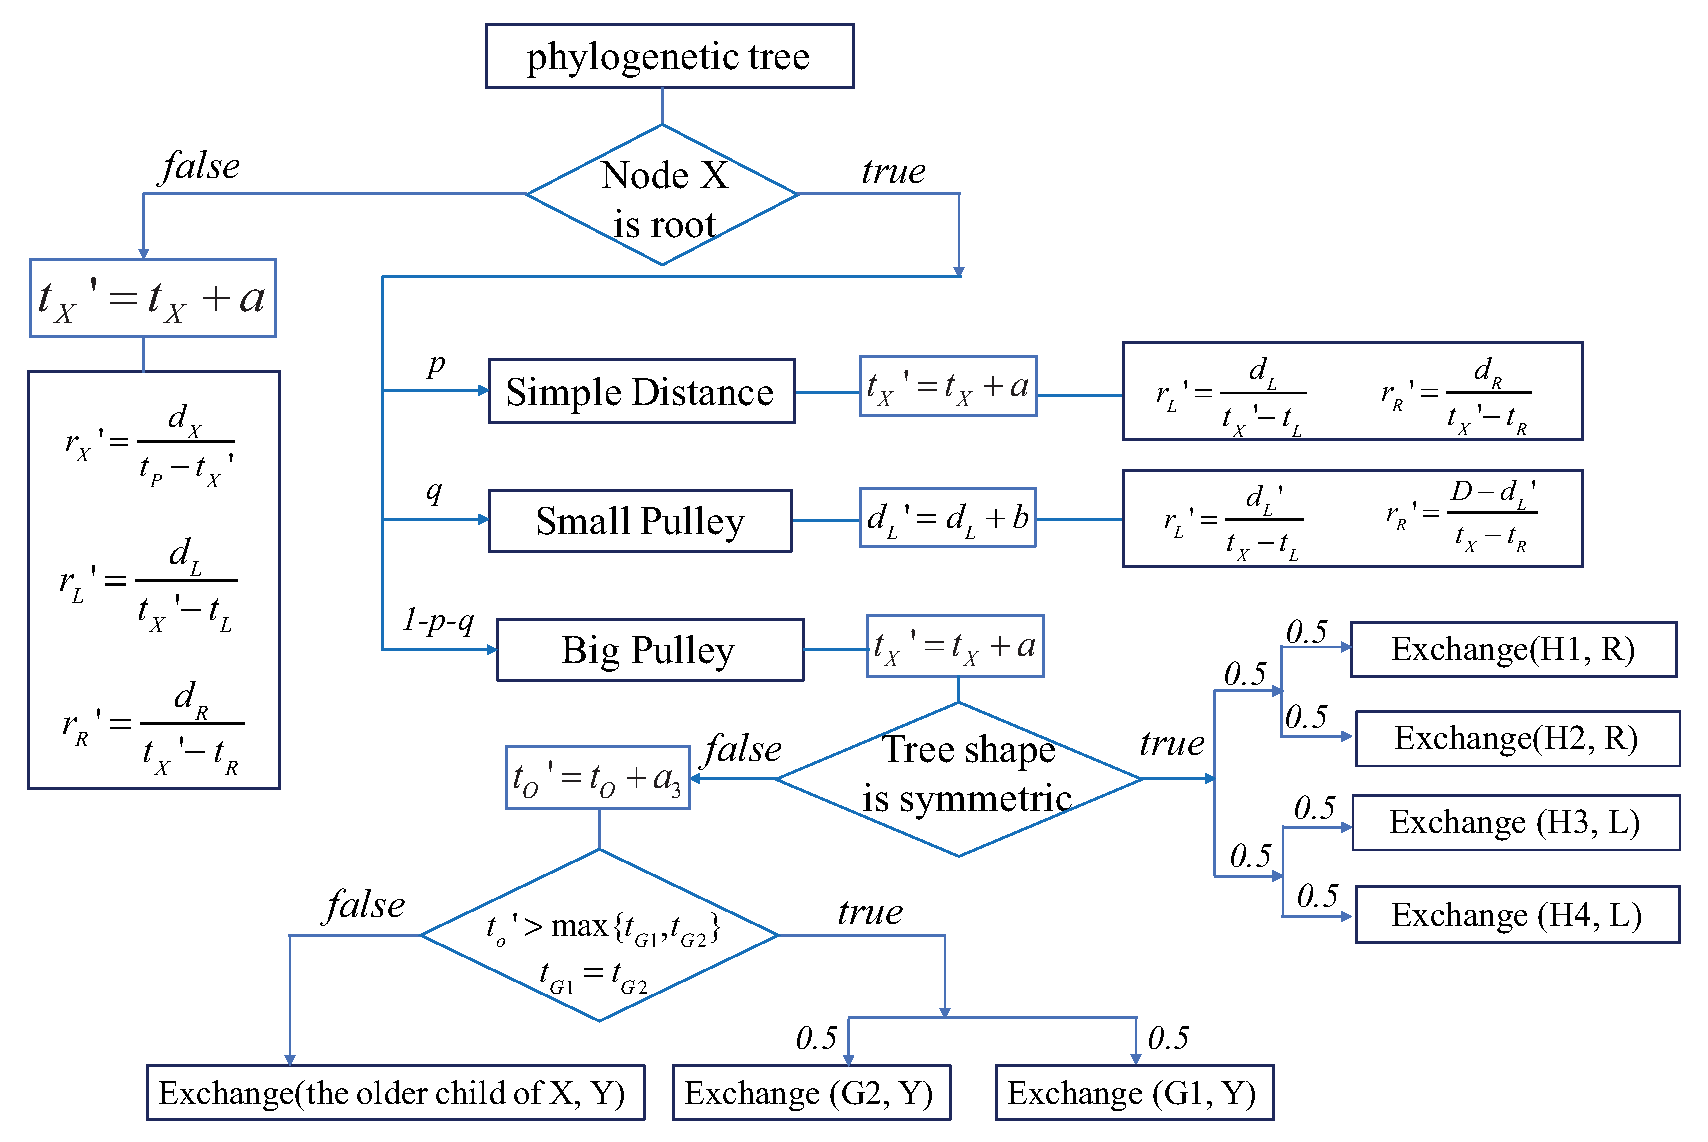
\includegraphics[width=12cm]{flowchart.eps}\\
\caption{\csentence{The flow chart of the constant distance operator.}}
\label{flowchart}
\end{figure}

\begin{figure}[h!]
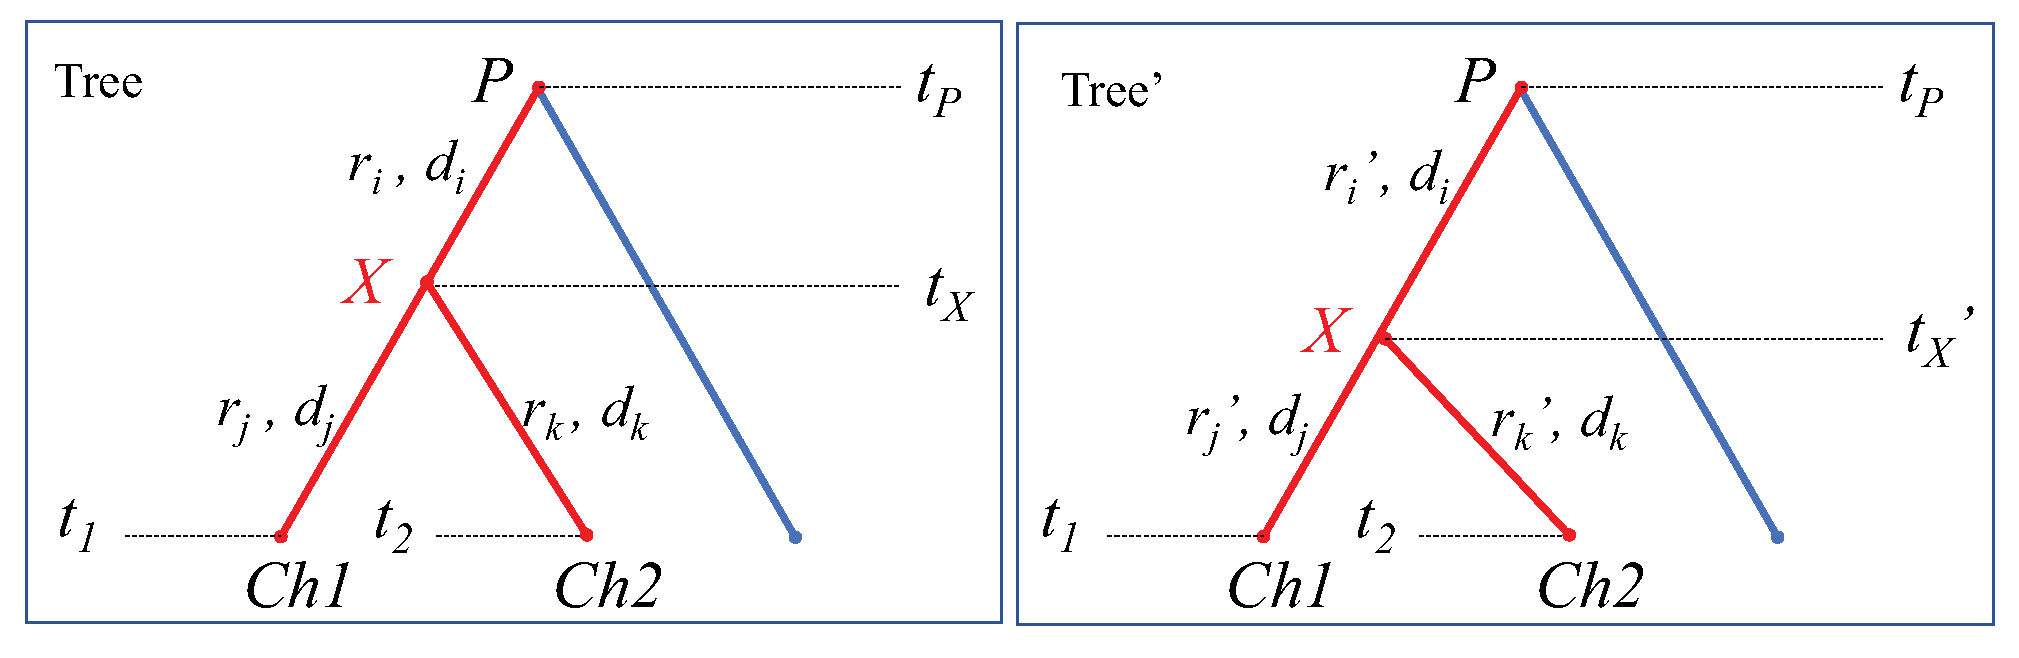
\includegraphics[width=12cm]{internalnodes.eps}\\
\caption{\csentence{The illustration of operations on internal nodes.}
             The operator proposes a tree ${g_{in}}'$ based on tree $g_{in}$, during which $d_i$, $d_j$, $d_k$ are constant.}
\label{internalnodes}
\end{figure}

\begin{figure}[h!]
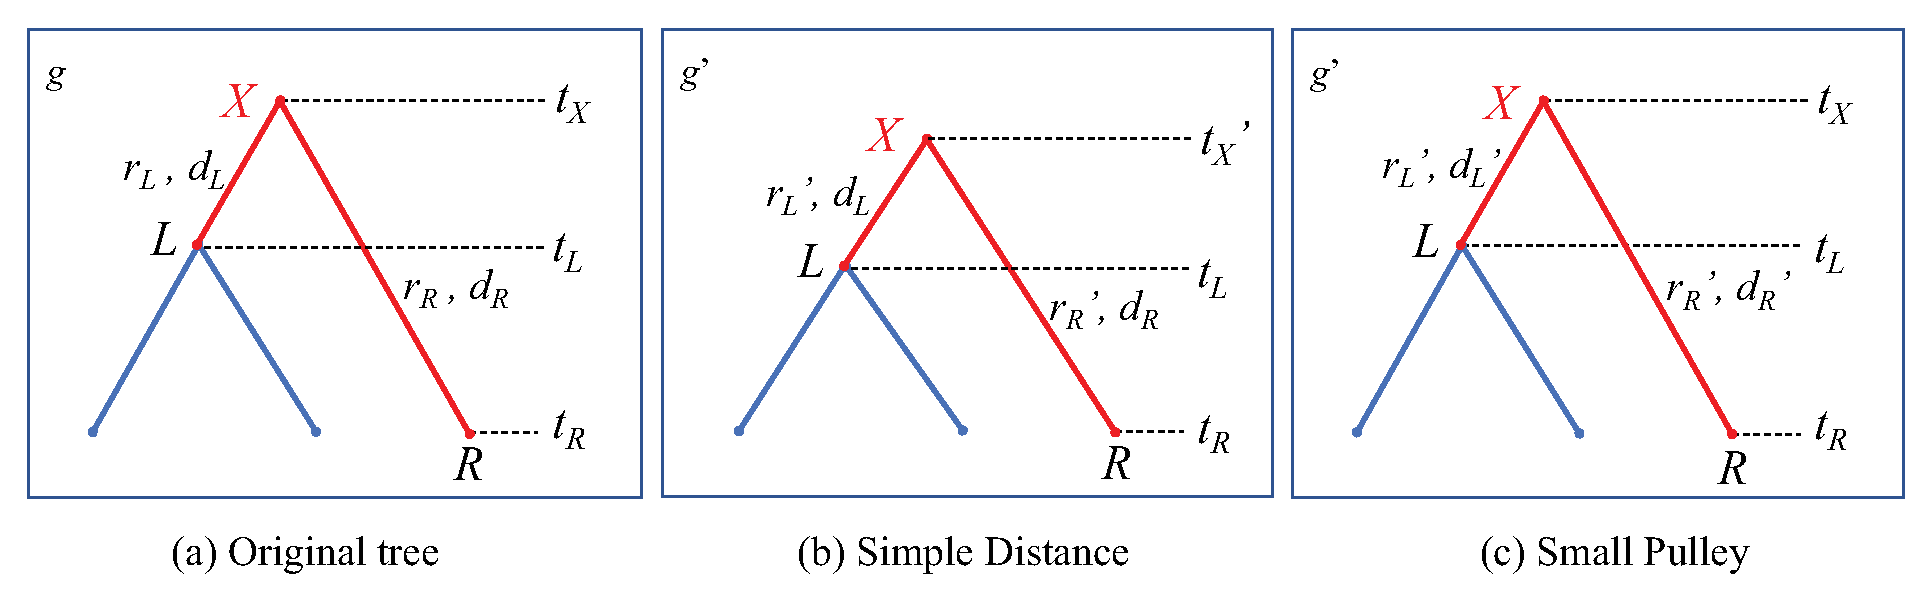
\includegraphics[width=12cm]{rootstrategy.eps}\\
\caption{\csentence{The illustration of Simple Distance and Small Pulley.}
             Simple Distance proposes ${g_{r1}}'$ and keeps $d_i$, $d_x$ constant. Small Pulley proposes ${g_{r2}}'$ and ${d_i} + {d_x}$ remains constant.}
\label{simpledistance}
\end{figure}


\begin{figure}[h!]
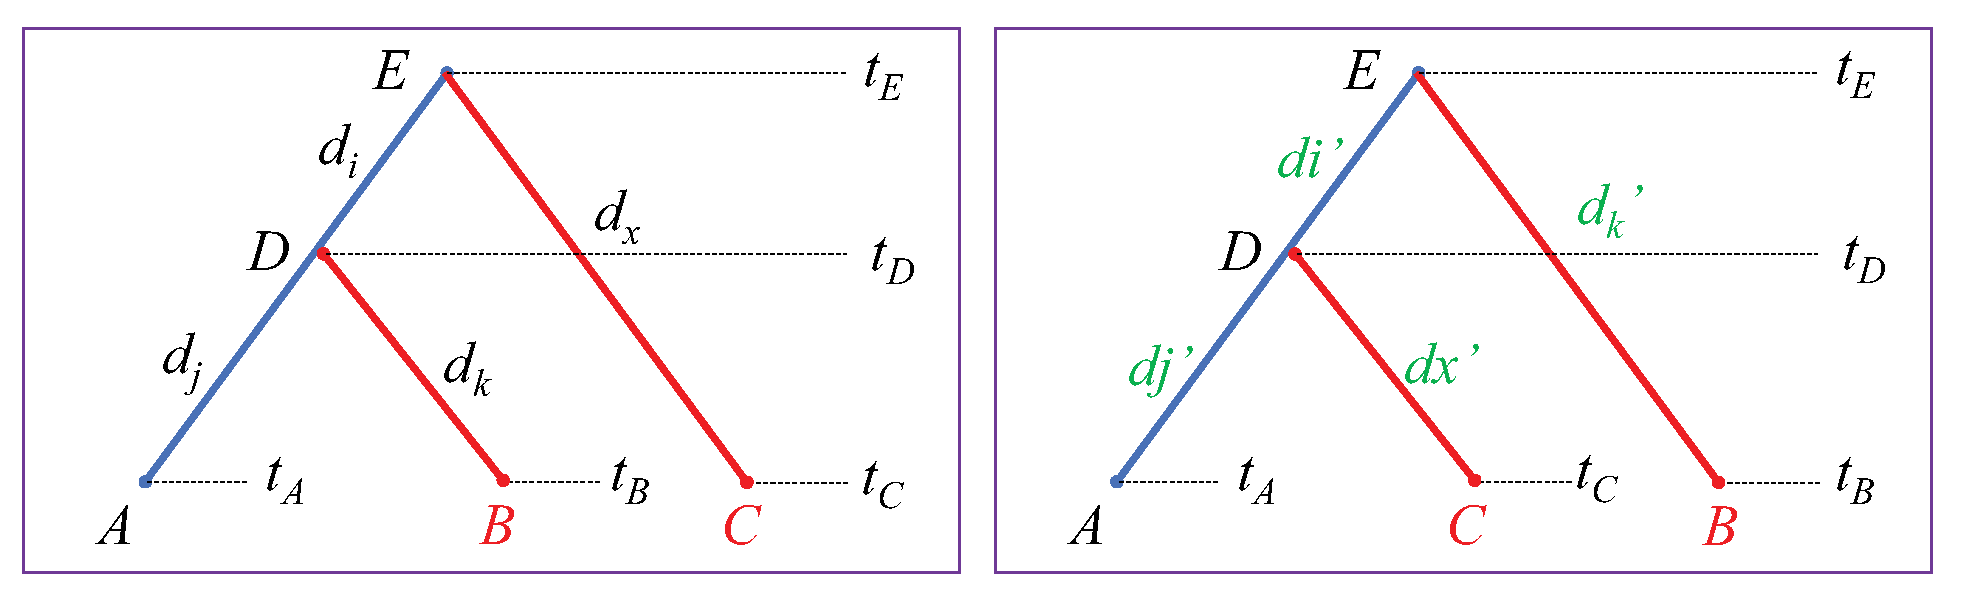
\includegraphics[width=12cm]{exchangemethod.eps}\\
\caption{\csentence{The illustration of \textit{Exchange (\textbf{Node1},\textbf{Node2})} method.}
             This method is applied to tree $g$ and proposes $g'$ by swapping \textbf{Node1} and \textbf{Node2}, so that the four distances are adjusted to maintain the distances among \textbf{Sib}, \textbf{Node1} and \textbf{Node2}.}
\label{exchangemethod}
\end{figure}

\begin{figure}[h!]
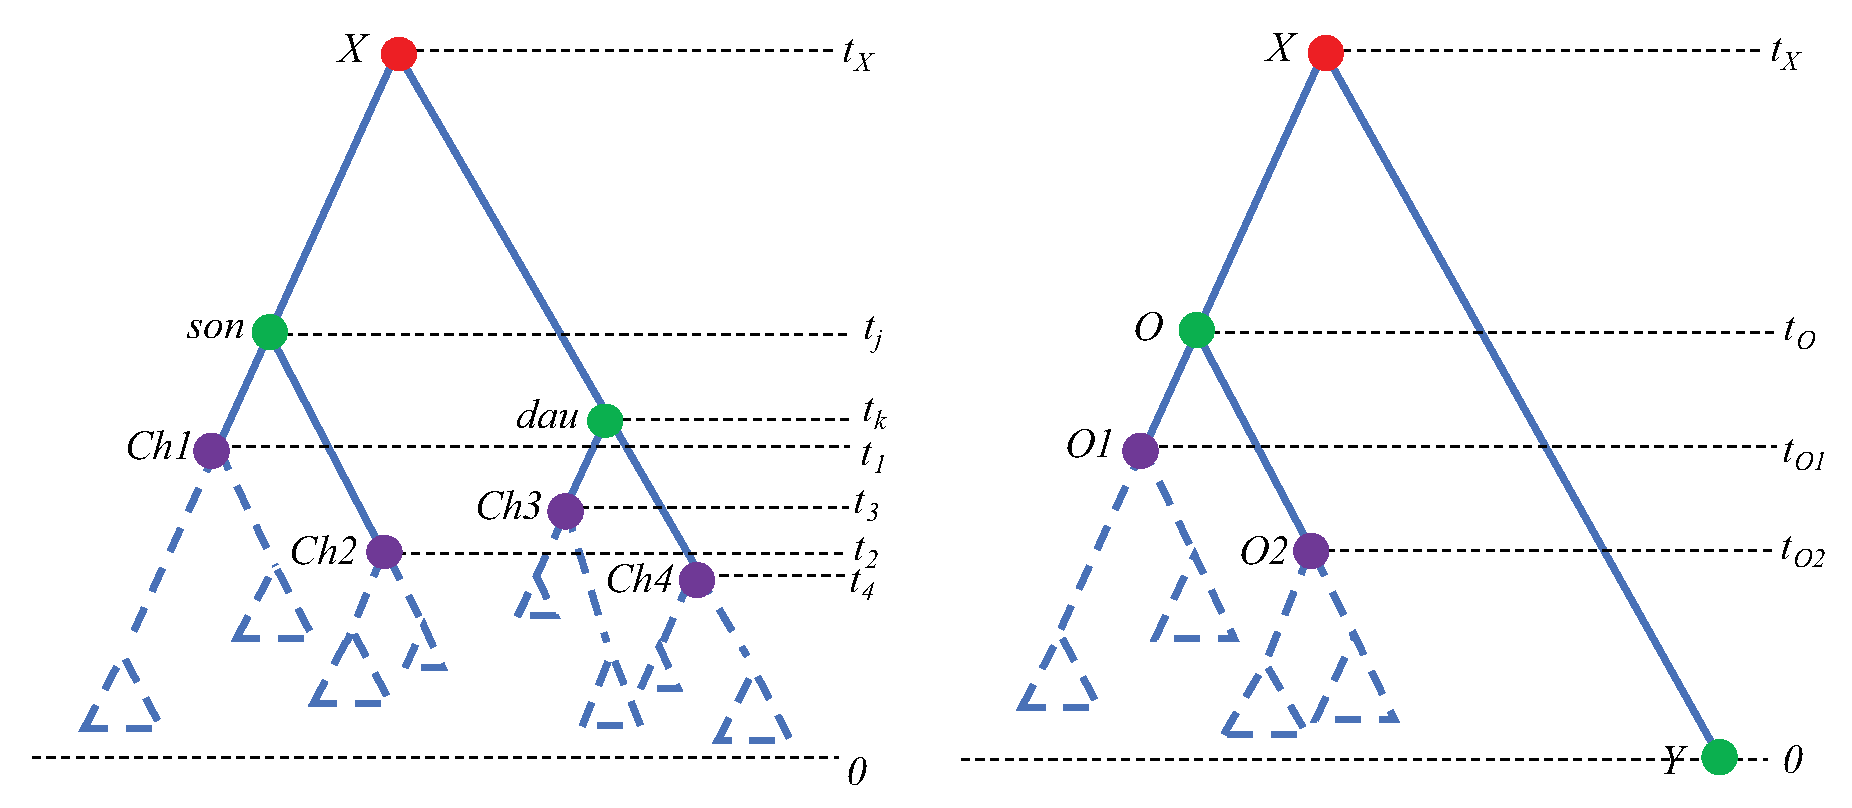
\includegraphics[width=12cm]{treeshape.eps}\\
\caption{\csentence{Two different tree shapes.}
             The symmetric tree is on the left and the asymmetric tree is on the right. The dashed triangles represent the potential subtrees rooted at the nodes.}
\label{treeshape}
\end{figure}

\begin{figure}[h!]
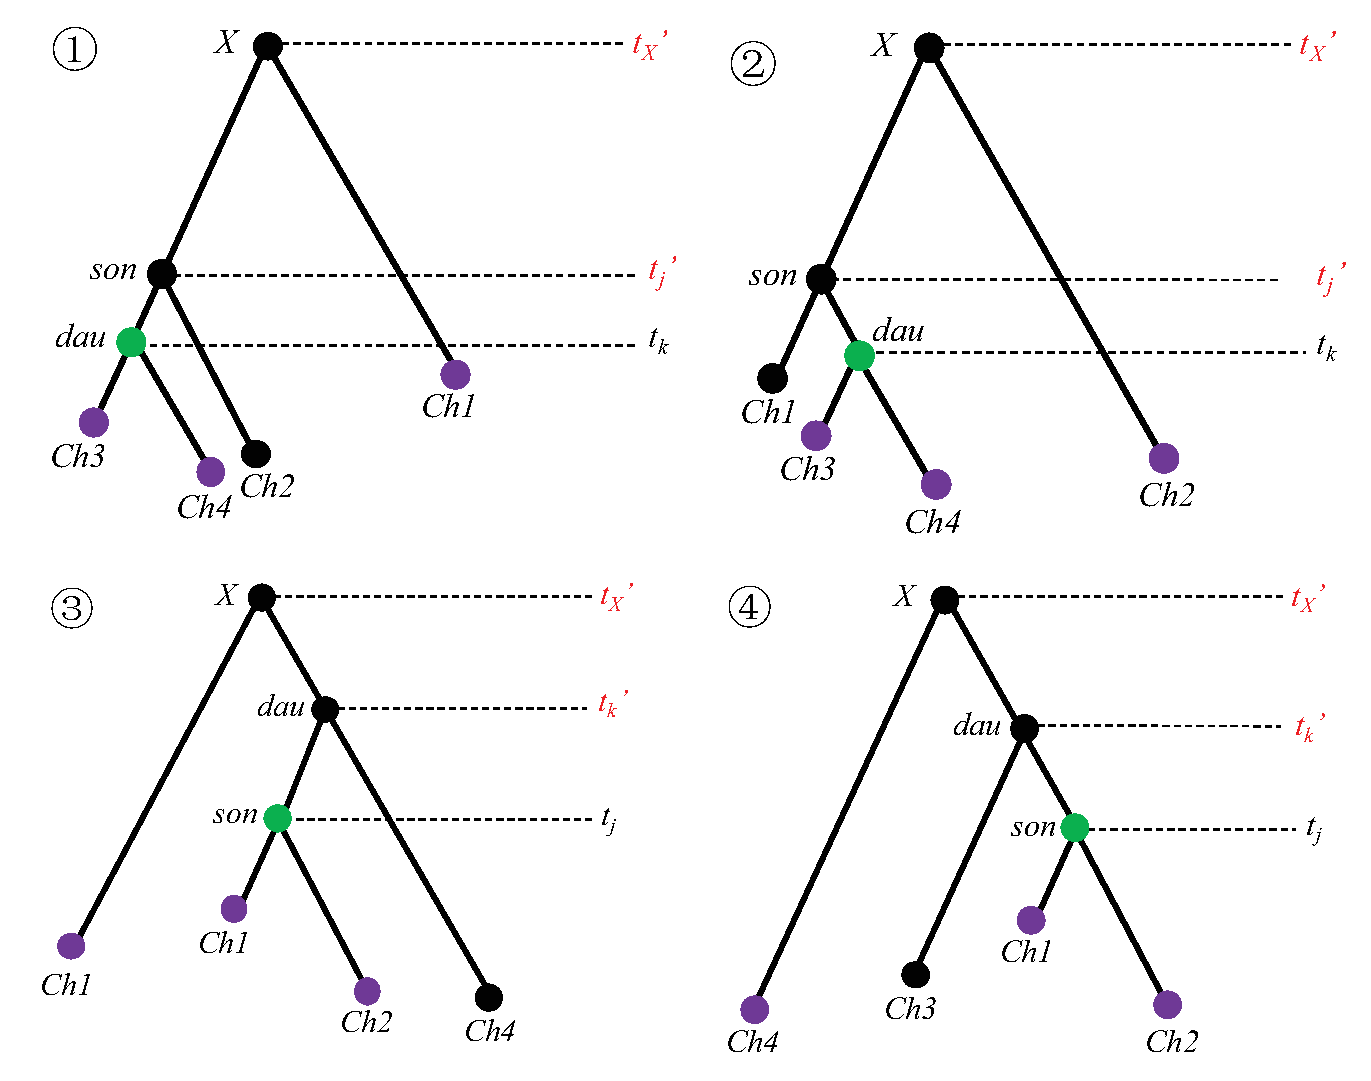
\includegraphics[width=12cm]{symmetric.eps}\\
\caption{\csentence{The illustration of operations on symmetric tree in Fig.\ref{treeshape}.}
             The proposed operator will propose one of the four possible trees, each with 0.25 probability.}
\label{symmetric}
\end{figure}

\begin{figure}[h!]
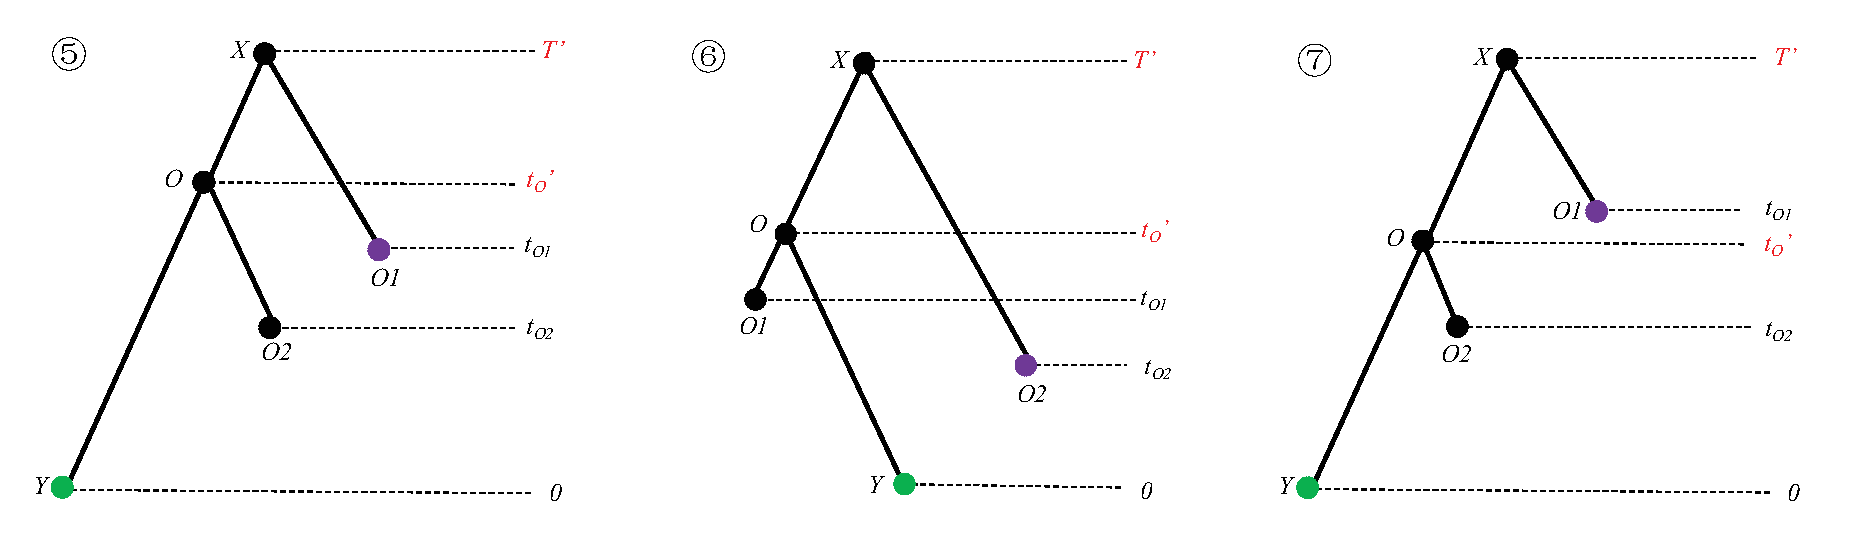
\includegraphics[width=12cm]{asymmetric.eps}\\
\caption{\csentence{The illustration of operations on asymmetric tree in Fig.\ref{treeshape}.}
             The proposed operator will propose one of the three possible trees. Depending on ${t_o}'$, \textcircled5 has 1 probability, \textcircled6 and \textcircled7 have 0.5 probability each.}
\label{asymmetric}
\end{figure}

\begin{figure}[h!]
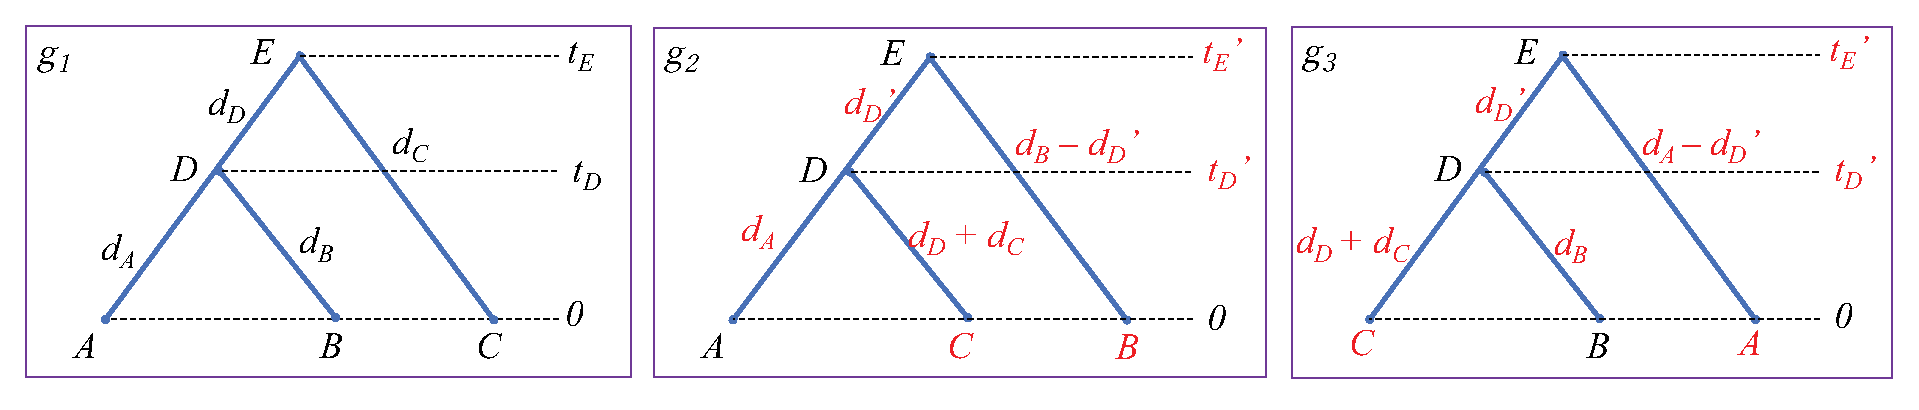
\includegraphics[width=12cm]{bigpulleyExp.eps}\\
\caption{\csentence{The illustration of sampling from prior.}
             $g_1$ is set to be the original tree where an MCMC chain starts. When testing Big Pulley, the proposed operator samples the trees among $g_1$, $g_2$ and $g_3$.}
\label{sampleprior}
\end{figure}

\begin{figure}[h!]
\centering
\subfigure[Senario 1: chain length = 10000000]{
\label{Fig.sub.1}
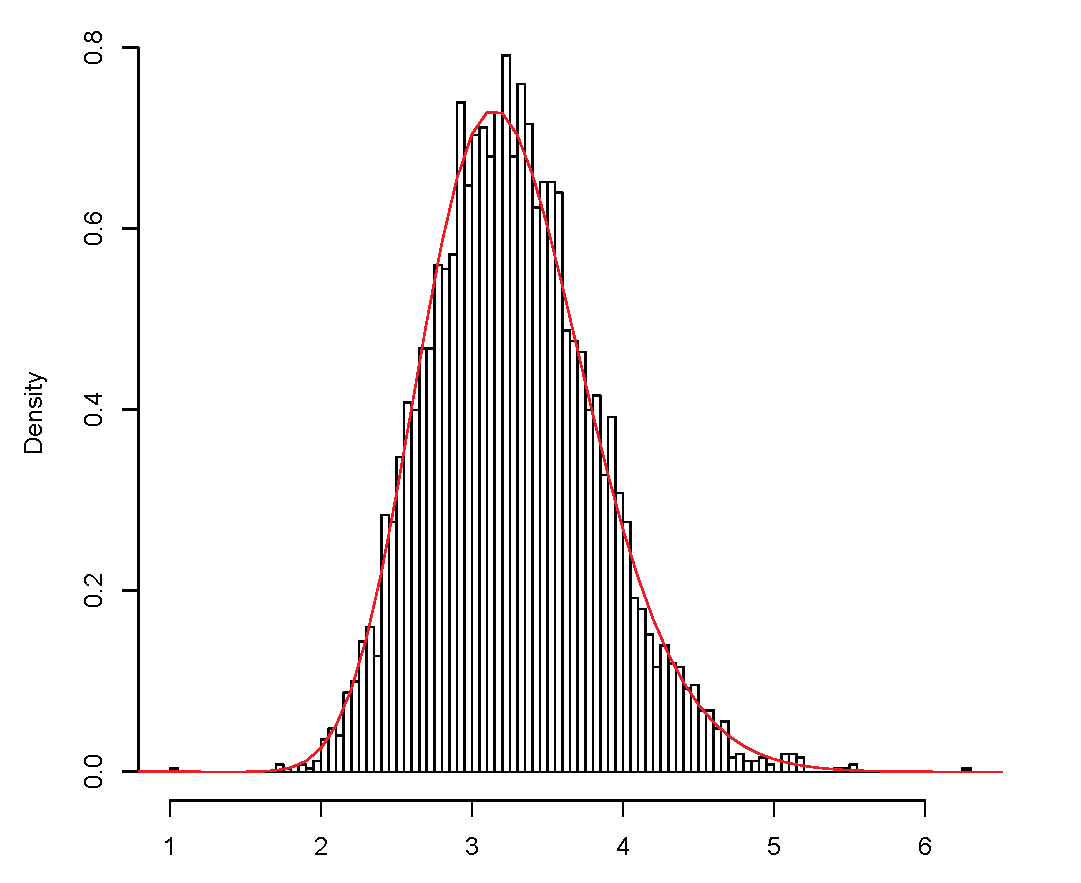
\includegraphics[width=0.45\textwidth]{Fig1}}
\subfigure[Senario 1: chain length = 20000000]{
\label{Fig.sub.2}
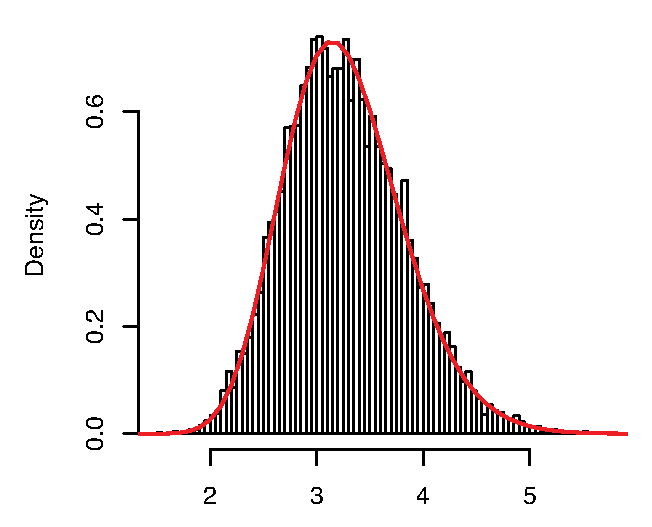
\includegraphics[width=0.45\textwidth]{Fig2}}
\subfigure[Senario 2: chain length = 10000000]{
\label{Fig.sub.3}
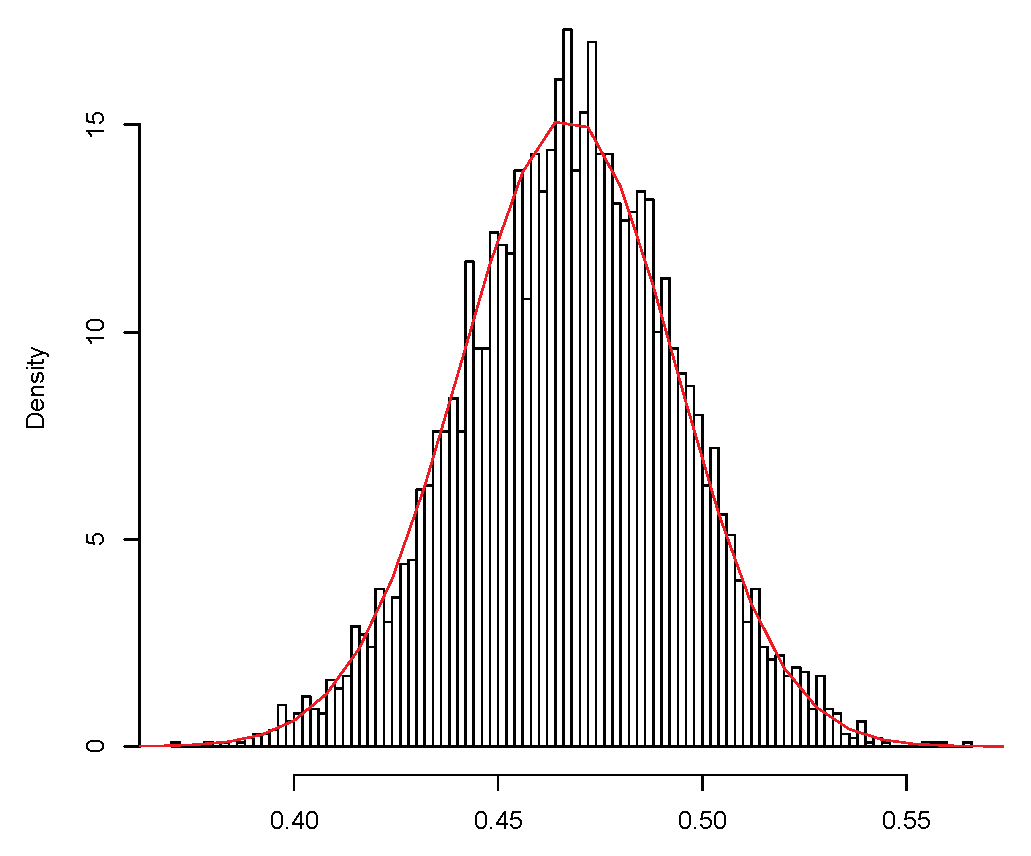
\includegraphics[width=0.45\textwidth]{Fig7}}
\subfigure[Senario 2: chain length = 20000000]{
\label{Fig.sub.4}
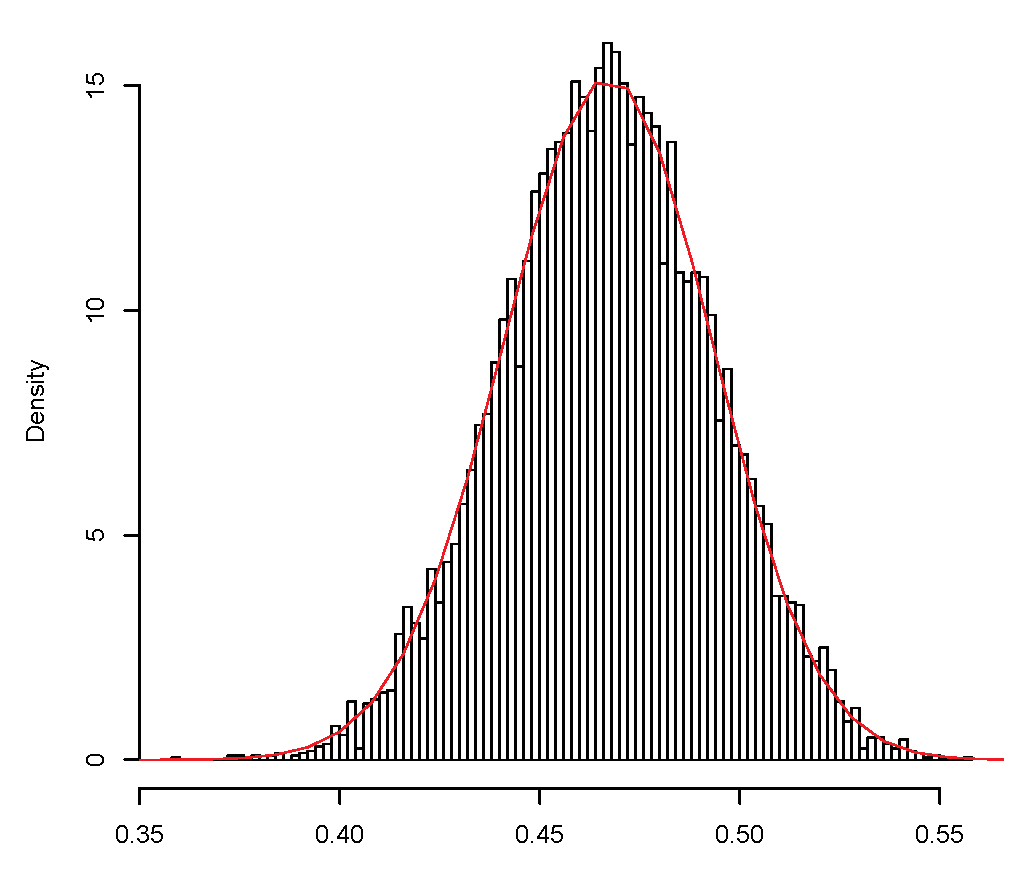
\includegraphics[width=0.45\textwidth]{Fig8}}
\caption{ \csentence{Sampled parameters in tests of internal nodes.}
             The horizontal axis represents the node time of D in Fig.\ref{sampleprior}. The two scenarios sample two trees with different distances specified in Table \ref{ini_inter} . And each scenario has two different lengths of MCMC chains.}
\label{res_int}
\end{figure}

\begin{figure}[h!]
\centering
\subfigure[$t_E$ in Simple Distance]{
\label{Fig.sub.5}
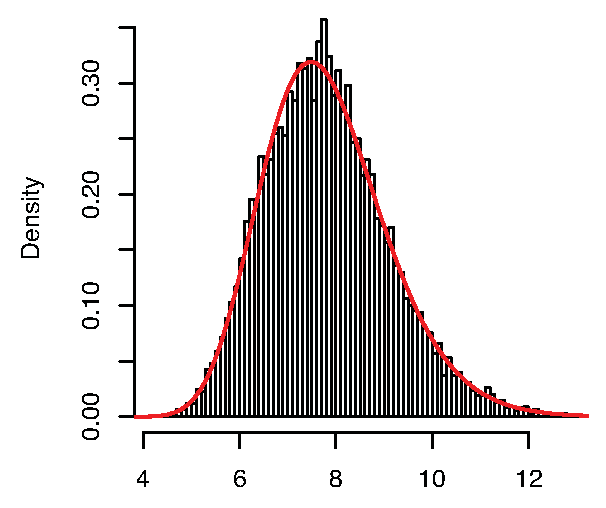
\includegraphics[width=0.35\textwidth]{RplotSD}}
\subfigure[$d_i$ in Small Pulley]{
\label{Fig.sub.6}
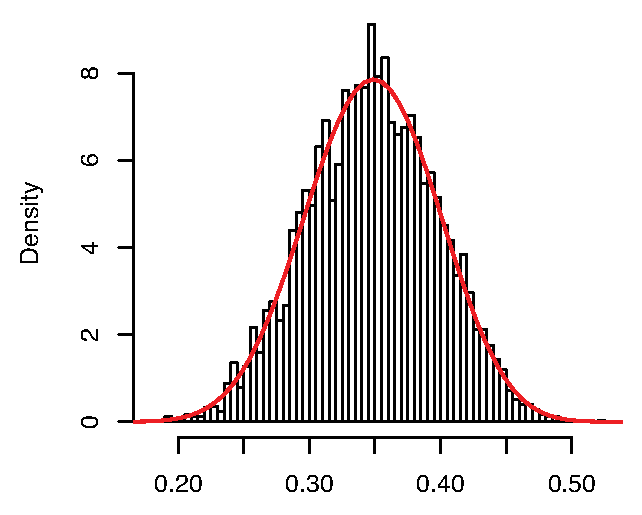
\includegraphics[width=0.35\textwidth]{RplotSP2}}
\subfigure[${d_i}$ in Big pulley]{
\label{Fig.sub.9}
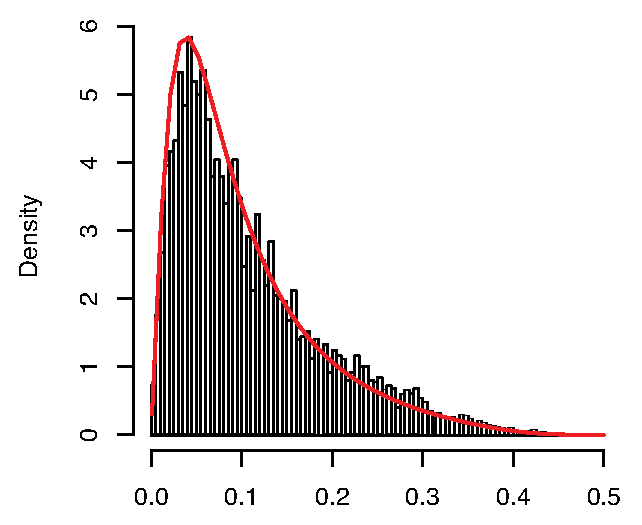
\includegraphics[width=0.35\textwidth]{bigd}}
\subfigure[${t_E}$ in Big pulley]{
\label{Fig.sub.10}
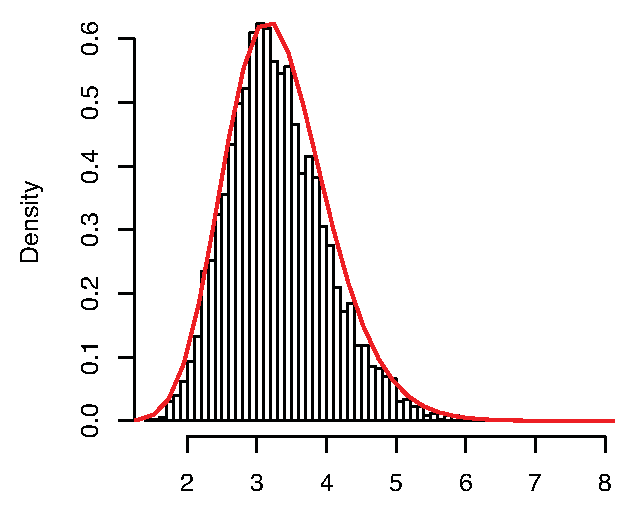
\includegraphics[width=0.35\textwidth]{bigT}}
\caption{\csentence{Sampled parameters in test of the root.}
             For the trees in Fig.\ref{sampleprior}, Simple Distance samples the root time $t_E$ only, Small Pulley samples the distance $d_i$ only, and Big Pulley samples $t_E$, $t_D$, $d_i$. To make it simple, $t_E$ and $d_i$ are compared.}
\label{res_roo1}
\end{figure}

\begin{figure}[h!]
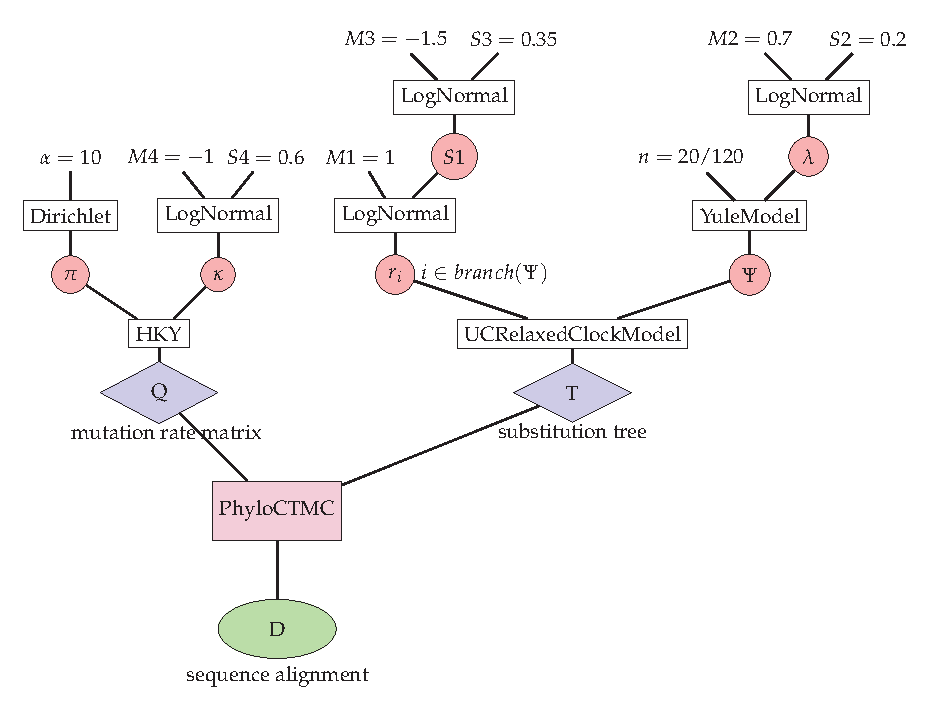
\includegraphics[width=12cm]{ModelValidation.eps}\\
\caption{\csentence{The models and prior distributions to simulate the sequence data.}
             The sequence alignment is simulated through a phylogenetic continuous-time Markov Chain that consists of a substitution model (HKY) and a uncorrelated relaxed clock model. The random variables in HKY model, including frequency and ratio, construct the mutation rate matrix. The rates and phylogenetic time trees specified by a Yule model construct the substitution tree. The standard deviation of rates and the birth rate in Yule model are both random variables following LogNormal distributions.}
\label{modelvalidation}
\end{figure}

\begin{figure}[h!]
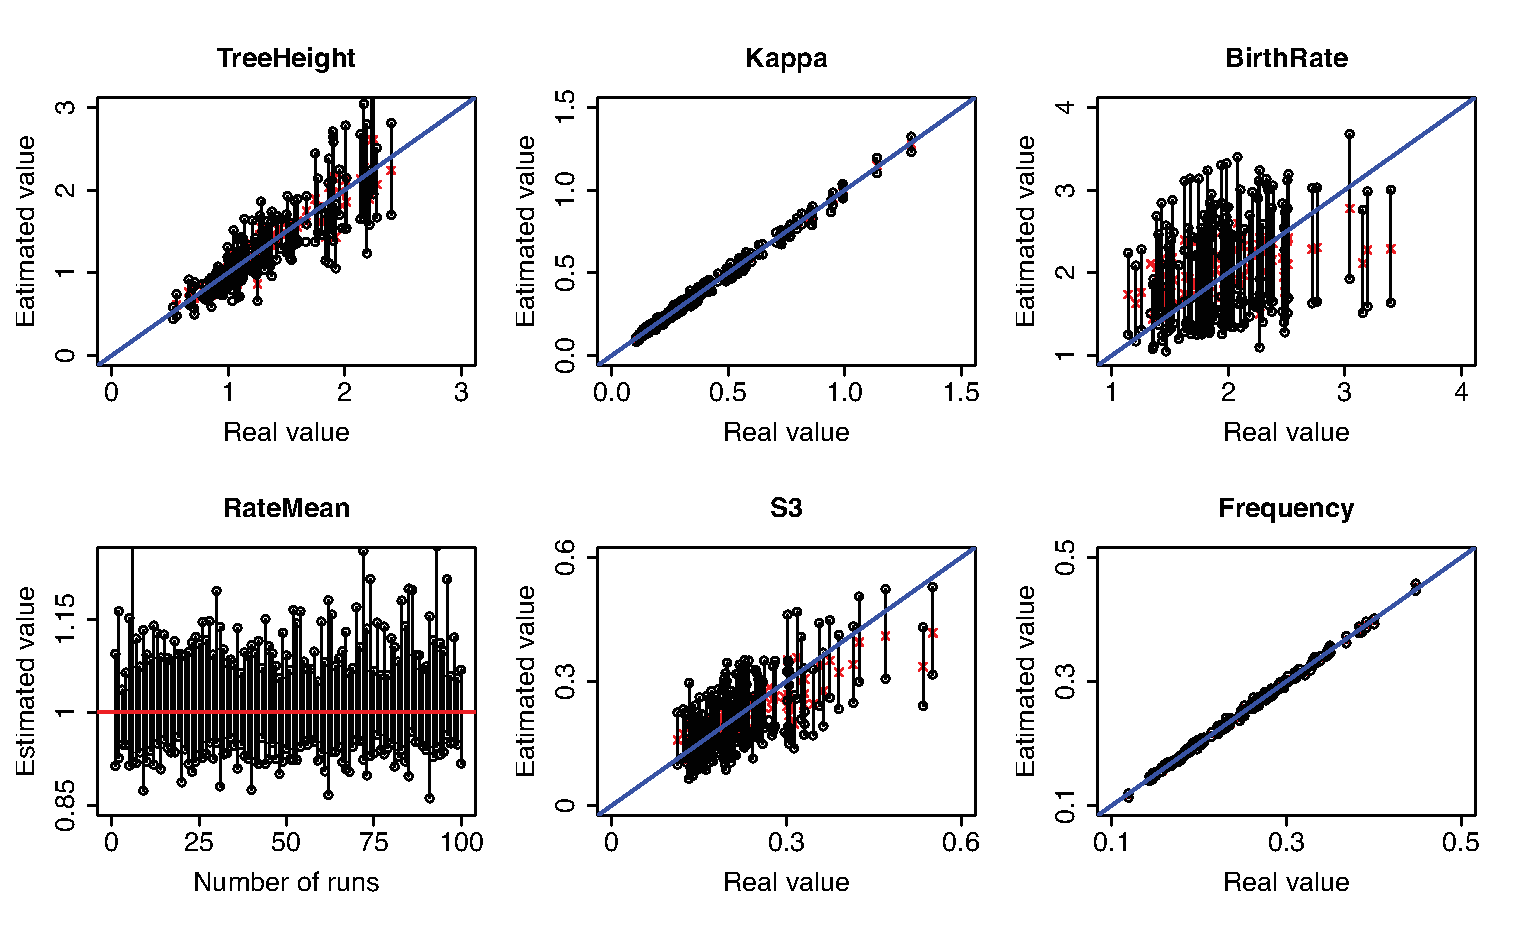
\includegraphics[width=12cm]{SmallTree.eps}\\
\caption{\csentence{Comparing the sampled parameters in simulation study with 20 taxa.}
             The red crossings represent the coordinates of real and estimated value. The vertical lines with circles show the 95\% HPD of the sampled parameters. The blue lines indicate that the estimated value is equal to the real value. The red line represents the fixed value of rate mean.}
\label{SmallTree}
\end{figure}

\begin{figure}[h!]
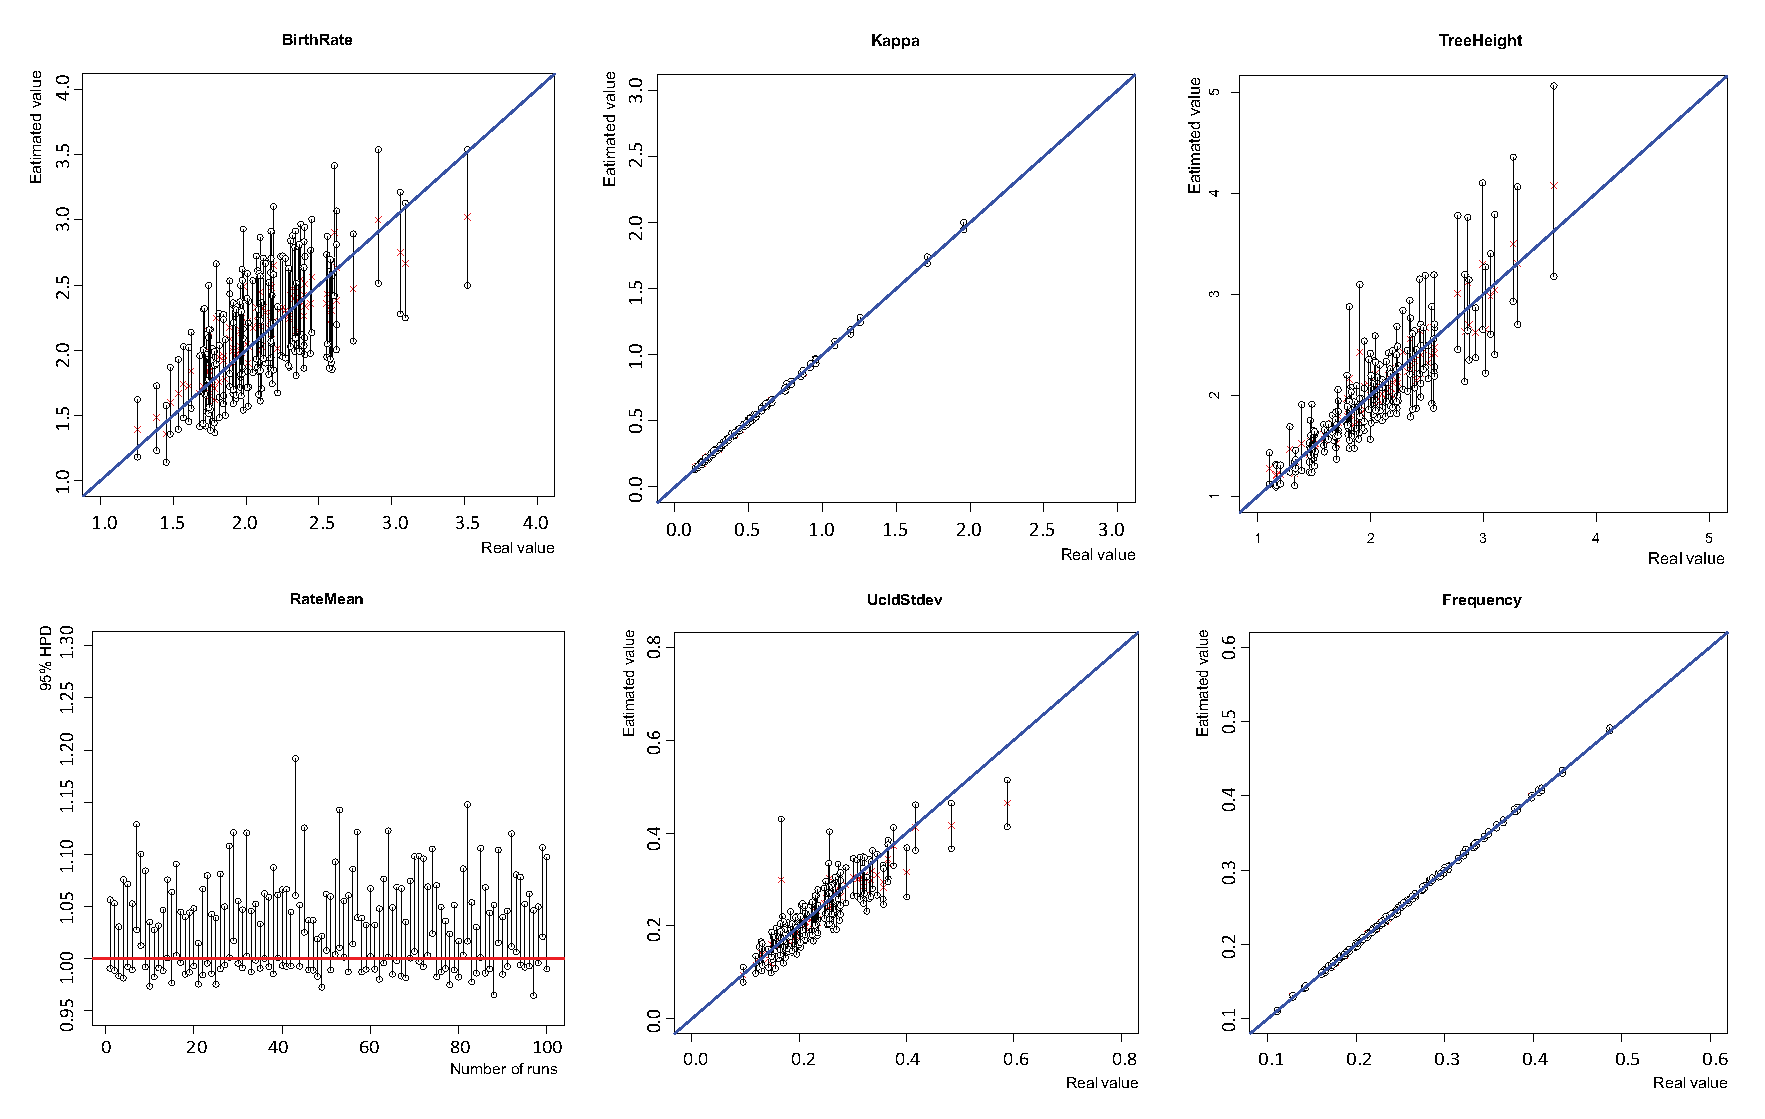
\includegraphics[width=12cm]{LargeTree.eps}\\
\caption{\csentence{Comparing the sampled parameters in simulation study with 120 taxa.}
             }
\label{LargeTree}
\end{figure}

\begin{figure}[h!]
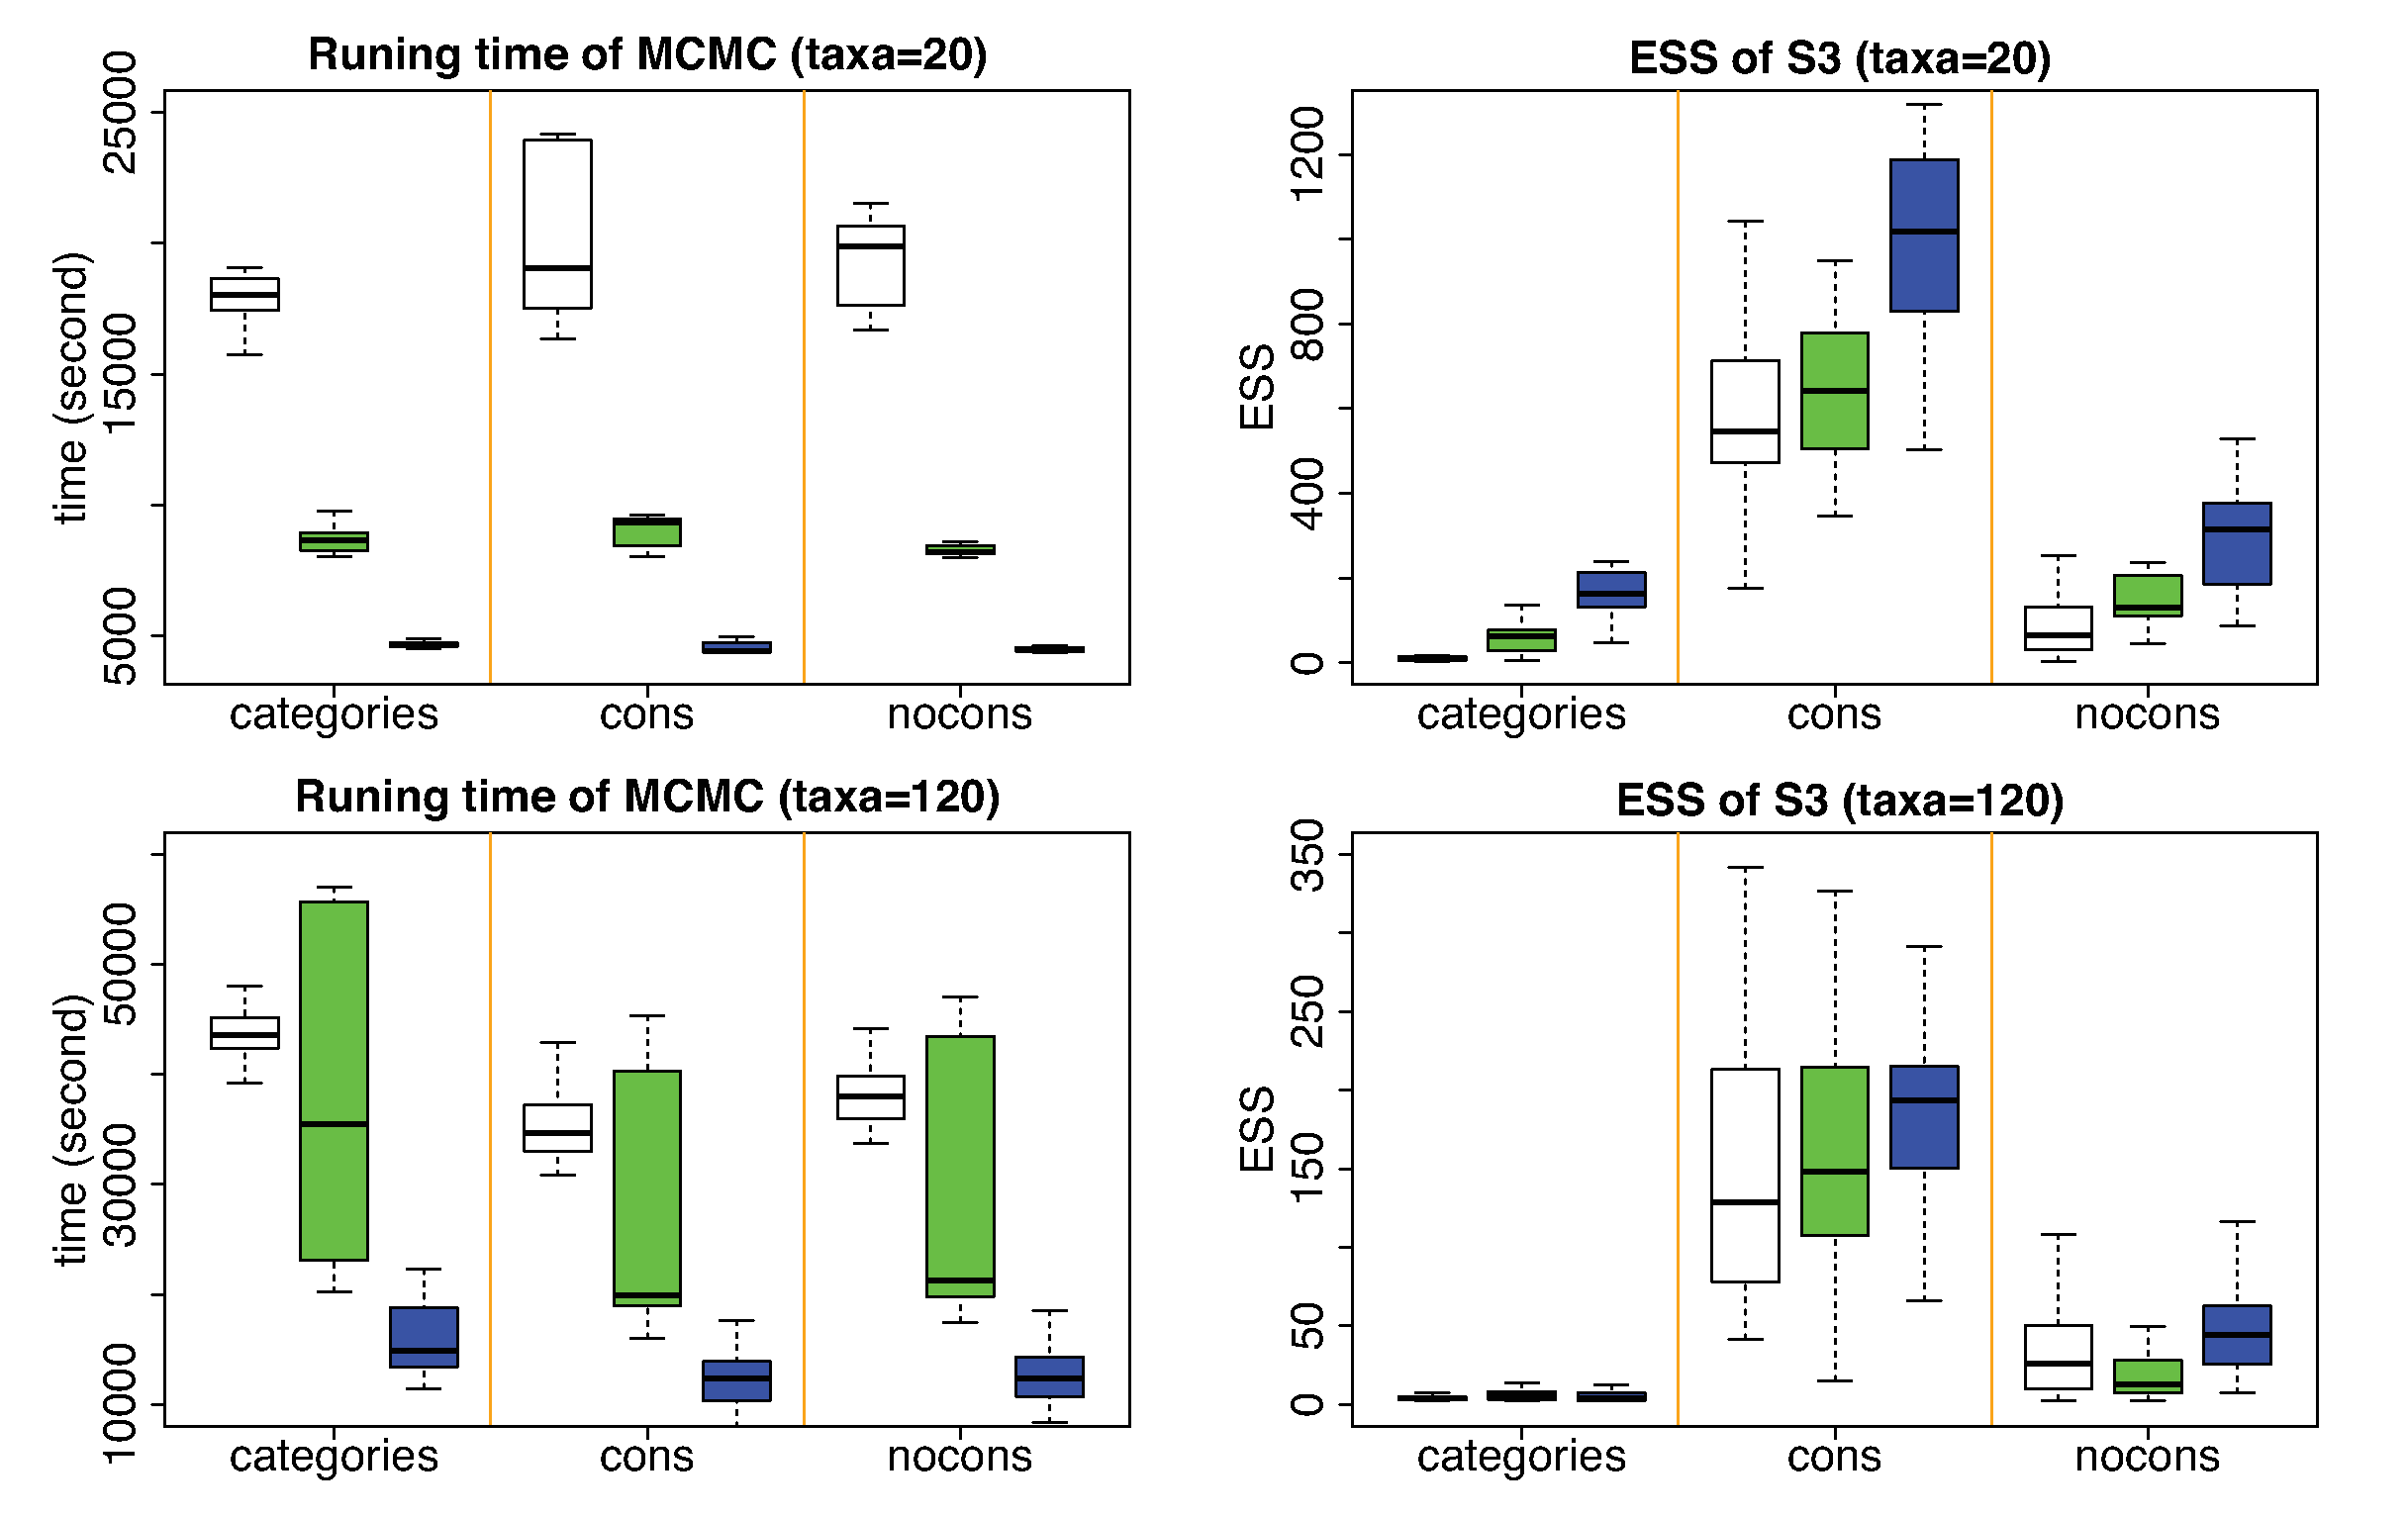
\includegraphics[width=12cm]{Efficiency.eps}\\
\caption{\csentence{Comparison of ESS and running time using simulated data.}
             The term long, medium and short represent the length of sequence with 20 thousand, 10 thousand and 5 thousand respectively.}
\label{eff_comp}
\end{figure}

\begin{figure}[h!]
\centering
\subfigure{
\label{P_ess}
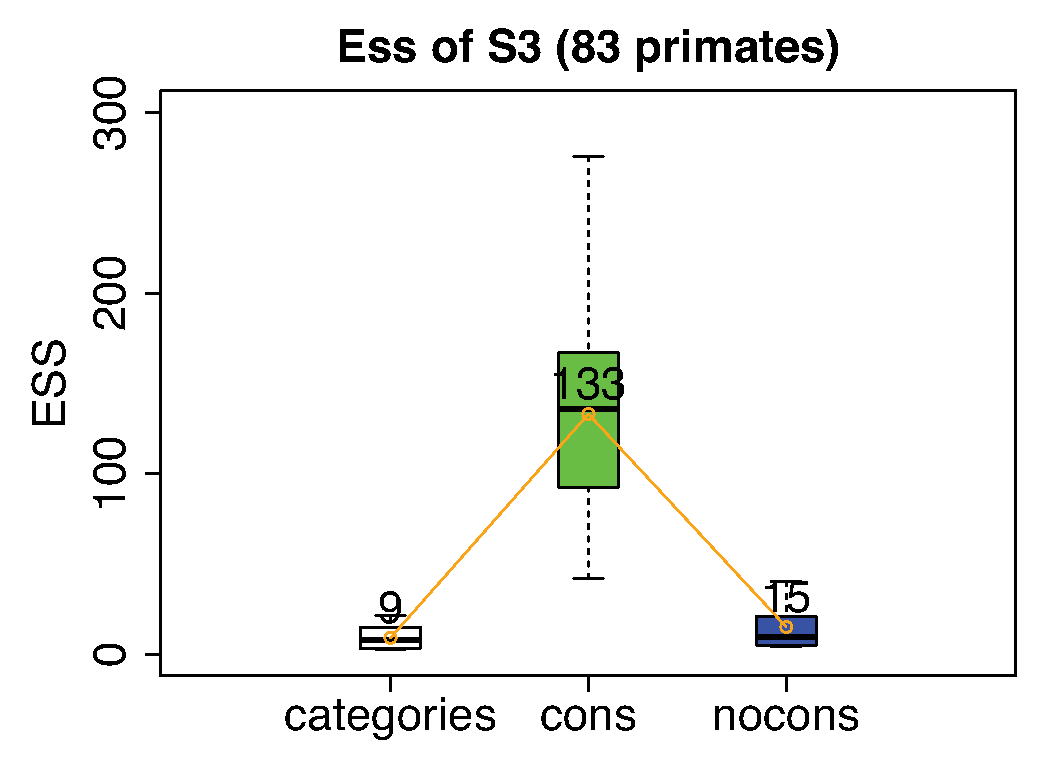
\includegraphics[width=0.45\textwidth]{primates2.eps}}
\subfigure{
\label{P_run}
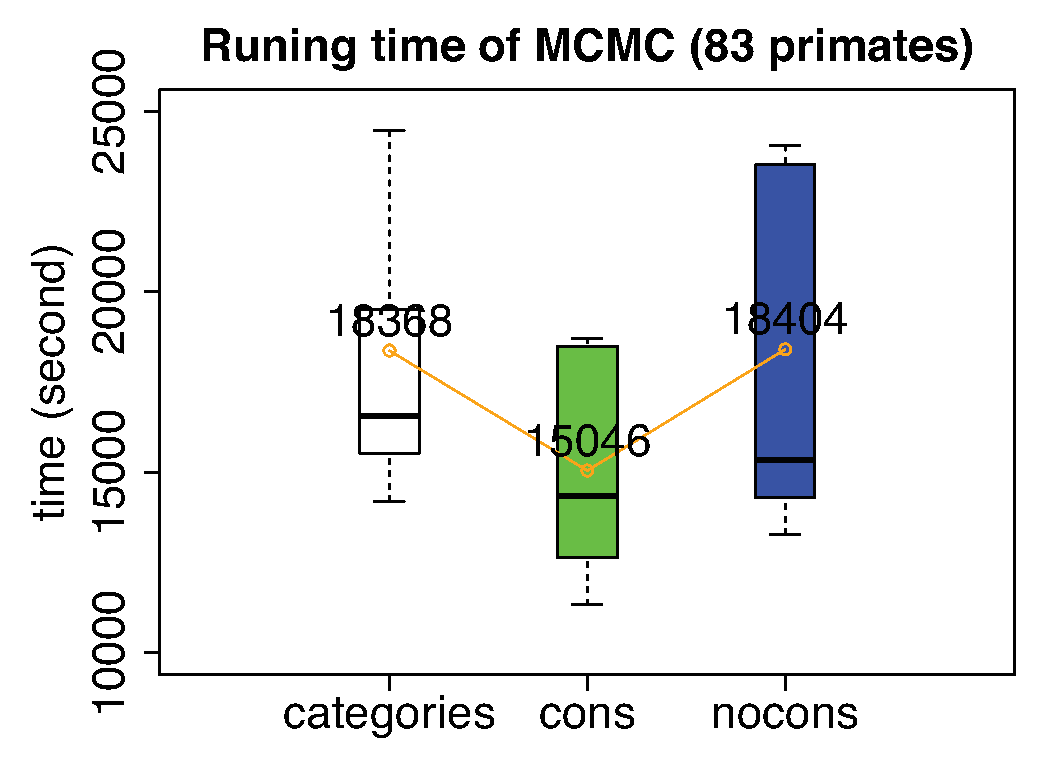
\includegraphics[width=0.45\textwidth]{primates1.eps}}
\caption{\csentence{Comparison of ESS and running time using primates data.}
             The orange curve links the mean values of each boxplot and the values are shown on the left of the boxplot.}
\label{eff_comp2}
\end{figure}

\begin{figure}[h!]
\centering
\subfigure[Clades]{
\label{Fig.sub.tree}
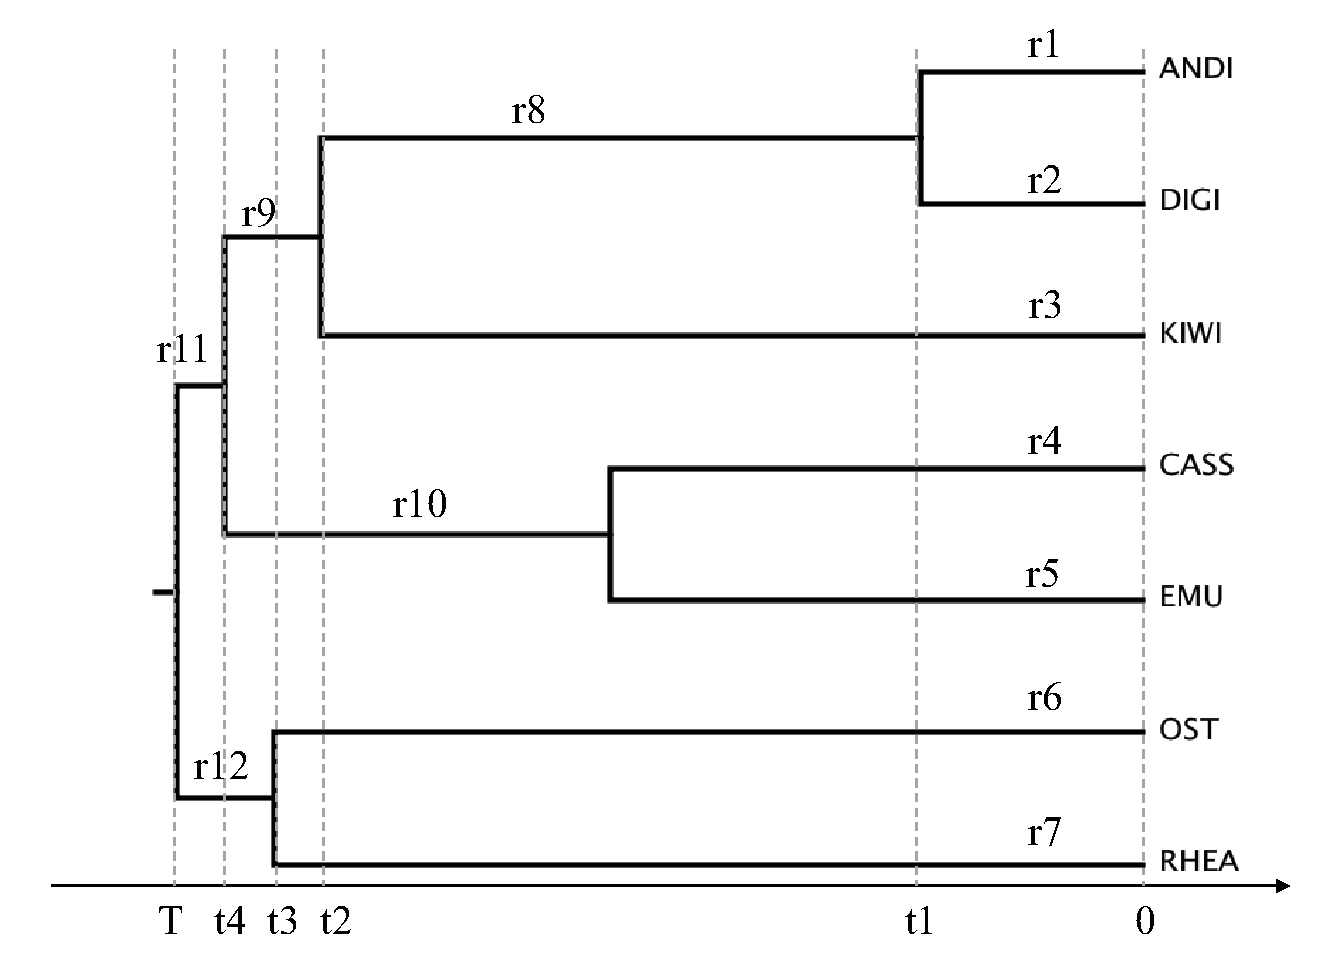
\includegraphics[width=0.5\textwidth]{correlationtree}}
\subfigure[Pairwise compare]{
\label{Fig.sub.correlation}
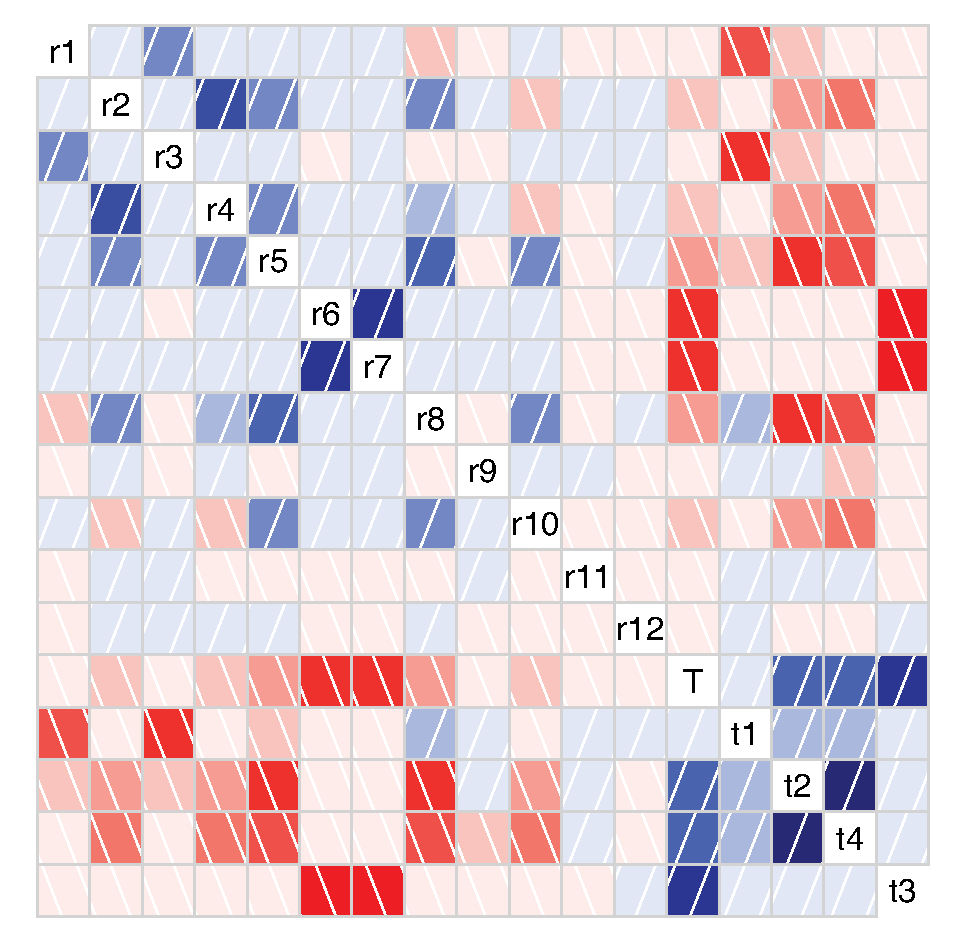
\includegraphics[width=0.4\textwidth]{rateandtime.eps}}
\caption{\csentence{Correlation between rates and node times in the ratites tree.}
             The rates and node times are in correspondence with the notations in Fig.\ref{summary3}. Blue indicates the positive relation and red indicates the negative relation. The darker the colour is, the stronger the relation tends to be.}
\label{correlation}
\end{figure}

\begin{figure}[h!]
\centering
\subfigure[Unrooted tree]{
\label{Fig.sub.11}
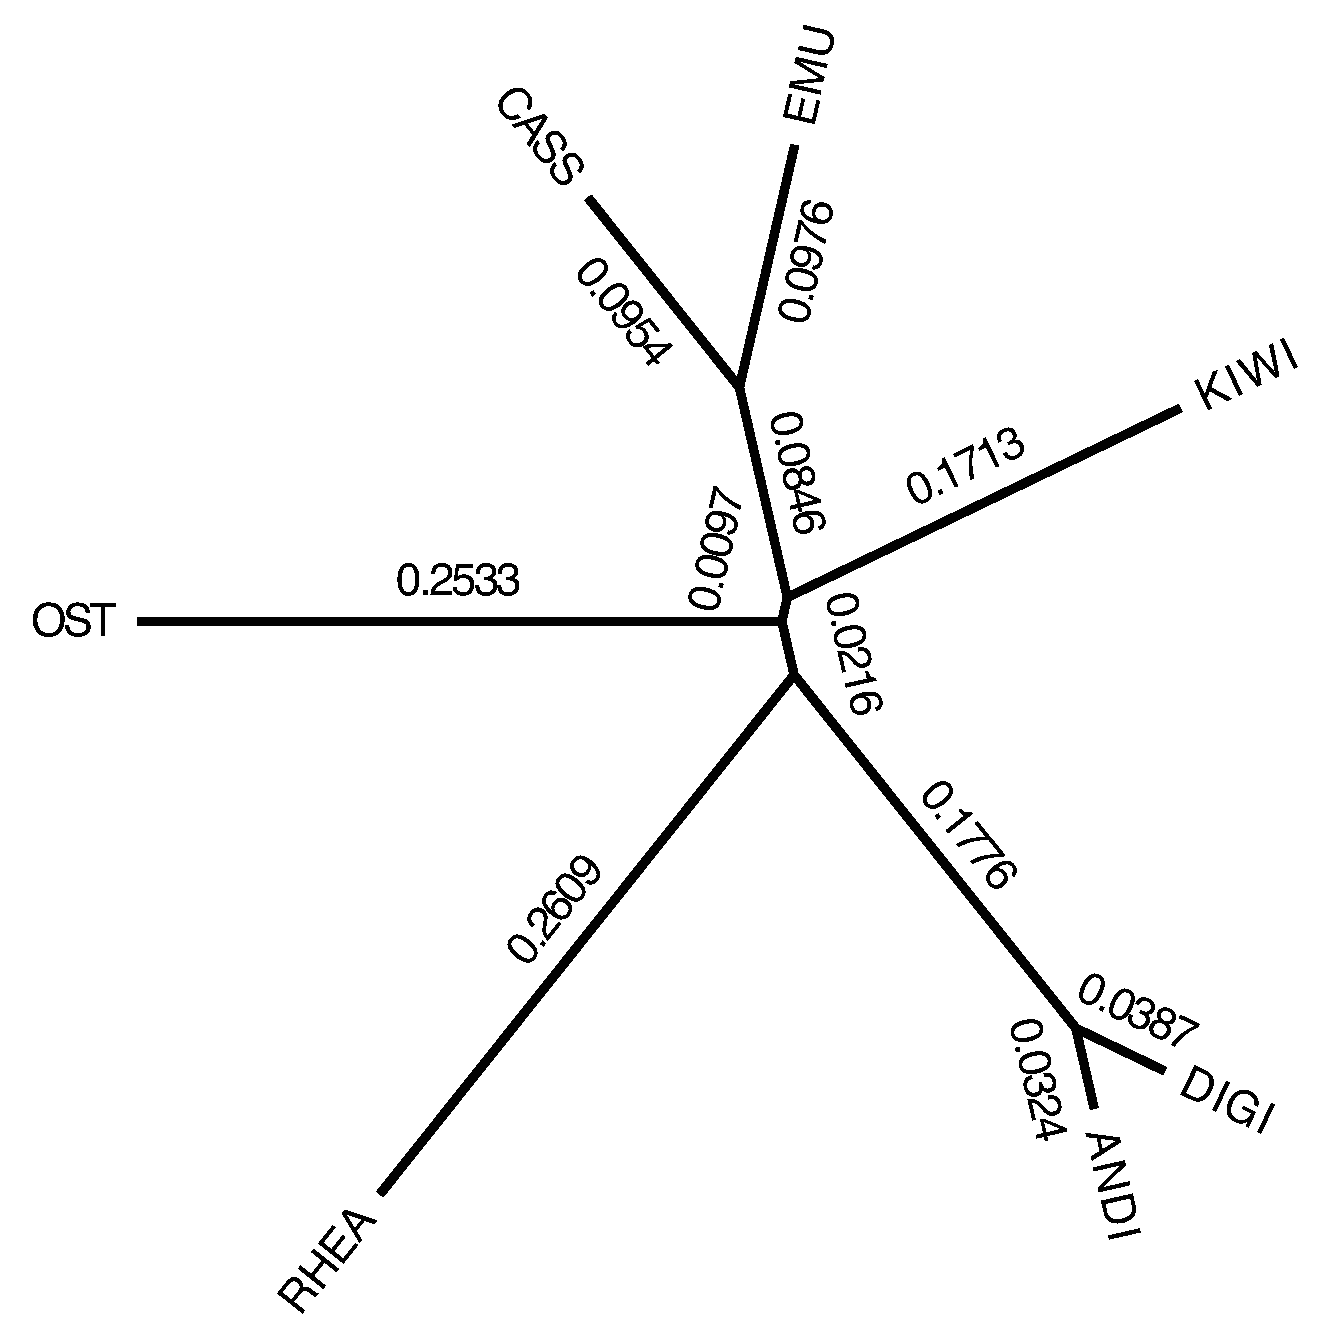
\includegraphics[width=0.35\textwidth]{unrootedtree}}
\subfigure[Rooted time tree]{
\label{Fig.sub.12}
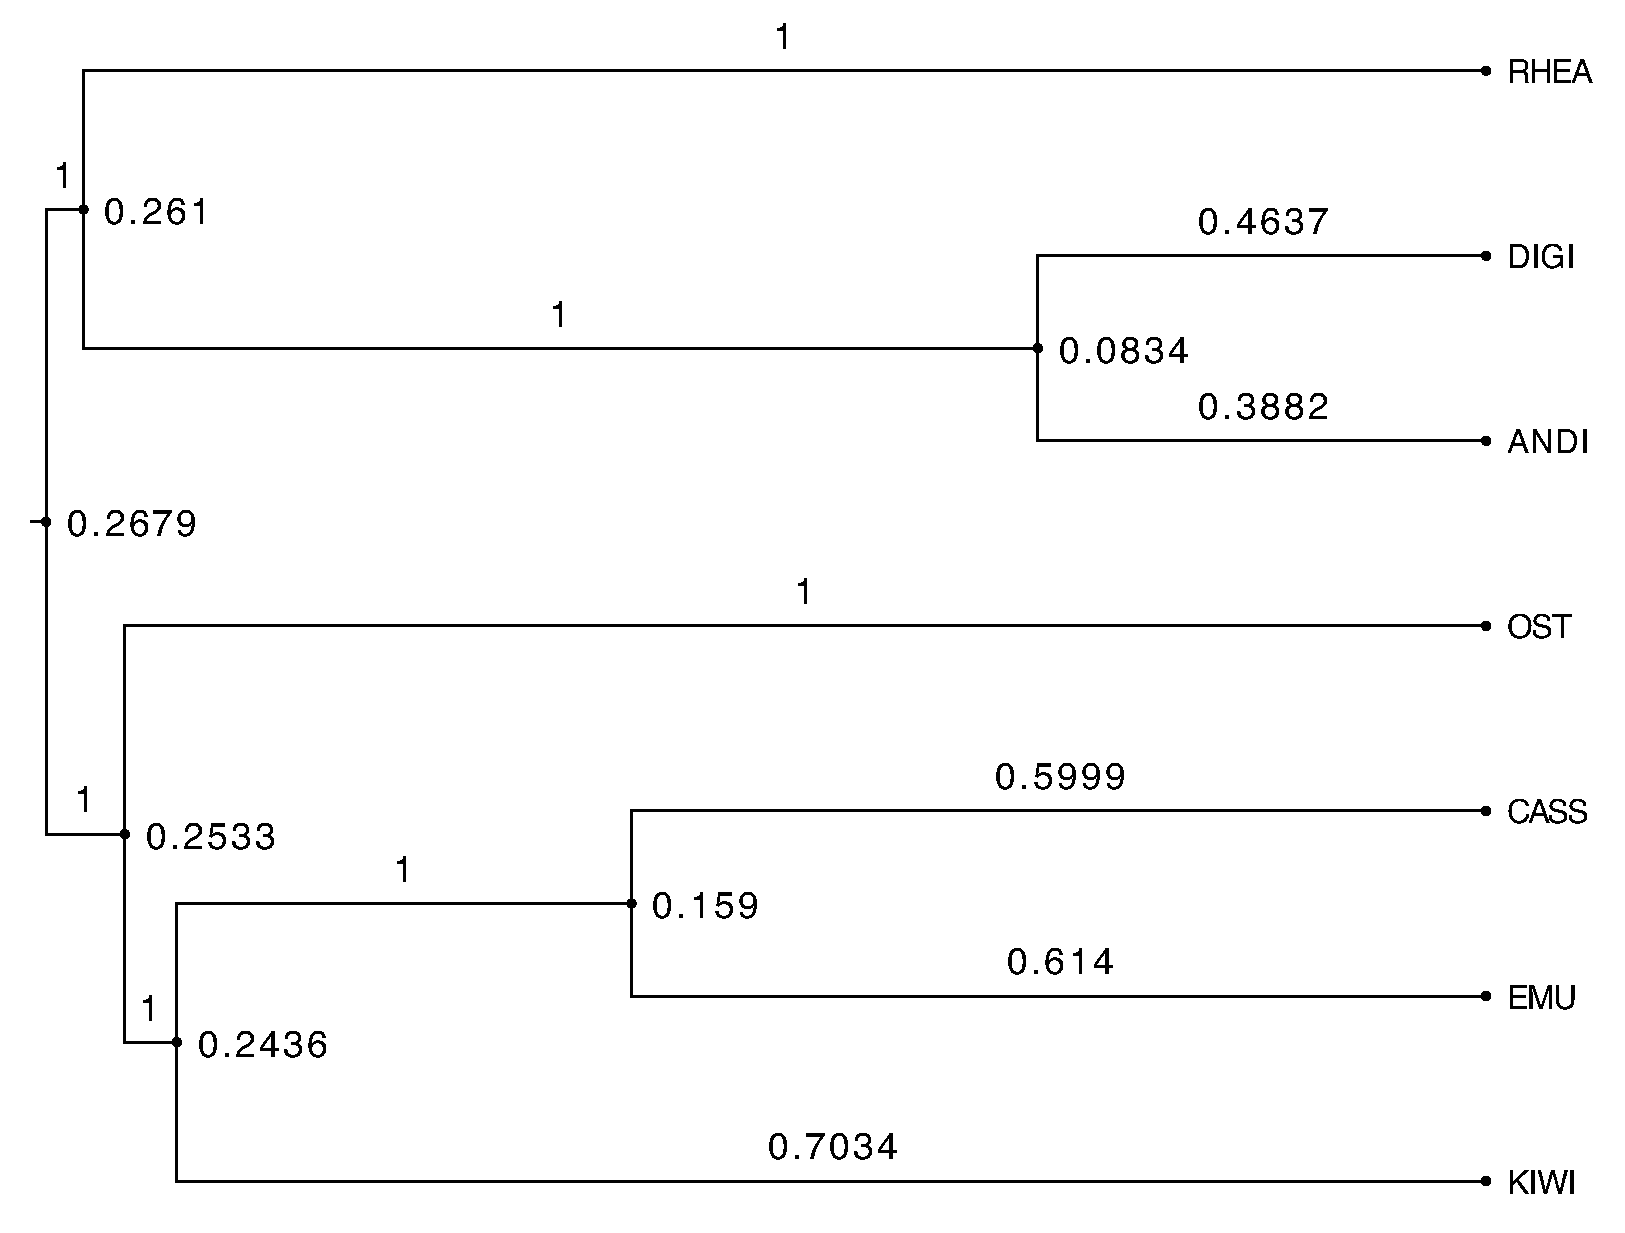
\includegraphics[width=0.4\textwidth]{initialtree}}
\subfigure[Summary tree of sampled trees]{
\label{summary3}
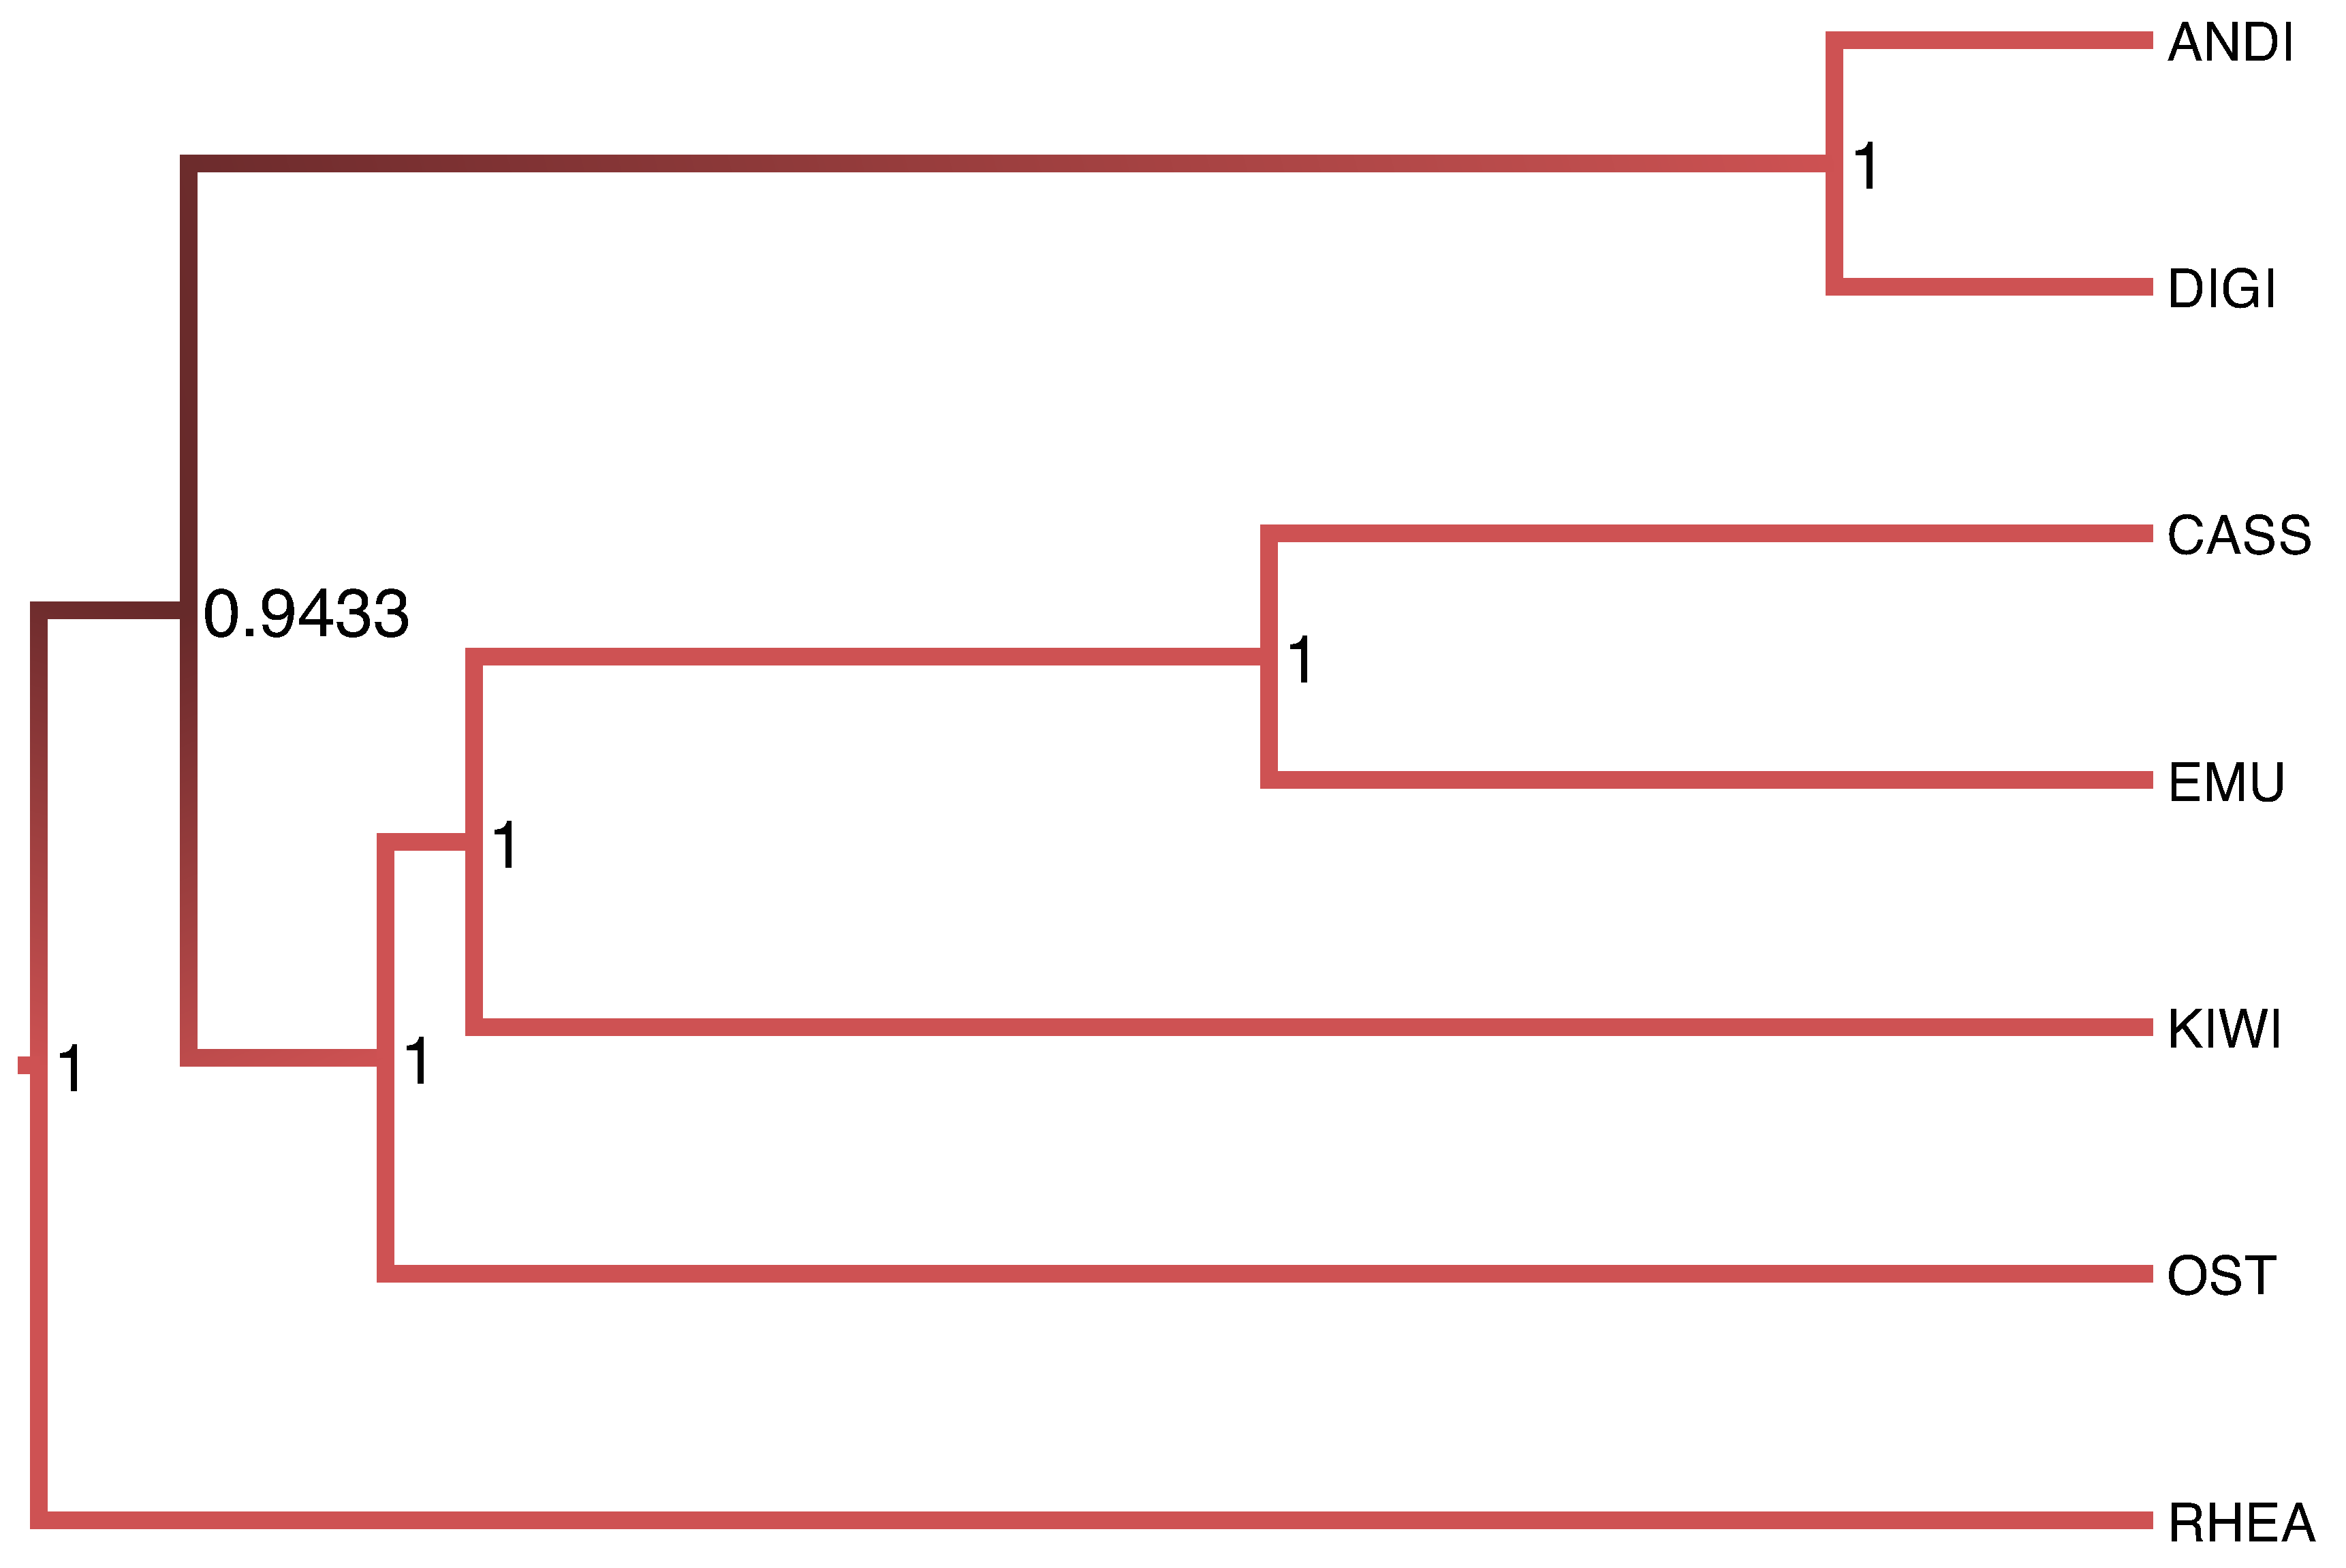
\includegraphics[width=0.4\textwidth]{summary3}}
\subfigure[Ratite phylogeography in Ref. \cite{cooper2001complete}]{
\label{ratites}
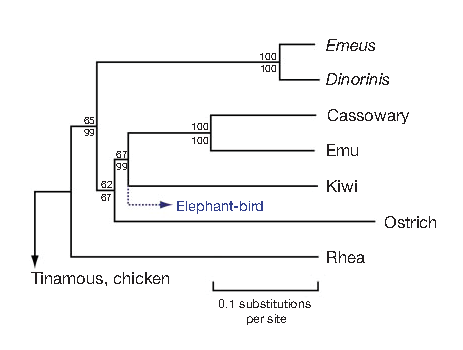
\includegraphics[width=0.45\textwidth]{ratites}}
\caption{\csentence{Illustration of sampling a fixed unrooted tree.}
            The unrooted tree is obtained from the ratites data set. The rooted time tree is the initial state in MCMC, with time on the nodes and rates on the branches.}
\label{withoutdata}
\end{figure}

\clearpage
%%%%%%%%%%%%%%%%%%%%%%%%%%%%%%%%%%%
%%                               %%
%% Tables                        %%
%%                               %%
%%%%%%%%%%%%%%%%%%%%%%%%%%%%%%%%%%%
%% Use of \listoftables is discouraged.
%%
\section*{Tables}
\begin{table}[h!]
  \centering
\begin{tabular}{c|cccc|c|c|cccc}
  \hline
&\multicolumn{4}{c|}{genetic distances (fixed)}&$t_D$&$t_E$&\multicolumn{4}{c}{initial rates}\\
&${d_j}$&${d_k}$&${d_x}$&${d_i}$&initial&(fixed)&${r_j}$&${r_k}$&${r_x}$&${r_i}$\\
\hline
Scenario 1&0.1&0.2&0.4&0.27&1&10&0.1&0.2&0.04&0.03\\
\hline
Scenario 2&0.4&0.8&2.4&1.6&0.4&0.8&1&2&3&4\\
  \hline
\end{tabular}
\caption{Initial settings for internal nodes}\label{ini_inter}
\end{table}

\begin{table}[h!]
  \centering
\begin{tabular}{c|c|ccc|ccc|c}
  \hline
&\multirow{2}*{Chain Length}&\multicolumn{3}{c|}{Sample from MCMC}&\multicolumn{3}{c|}{R curve}&Plot\\
&~&Mean&Err&StdEv&Mean&Err&StdEv&\\
\hline
\multirow{2}*{Senario 1}&10000000&3.2727&8.3e-3&0.5467&\multirow{2}*{3.2669}&\multirow{2}*{1.3e-06}&\multirow{2}*{0.5553}&Fig.\ref{Fig.sub.1}\\
~&20000000&3.271&6.1e-3&0.5616&~&~&~&Fig.\ref{Fig.sub.2}\\
\hline
\multirow{2}*{Senario 2}&10000000&0.4677&3.9e-04&0.0265&\multirow{2}*{0.4667}&\multirow{2}*{3.5e-05}&\multirow{2}*{0.0262}&Fig.\ref{Fig.sub.3}\\
~&20000000&0.4672&2.8e-04&0.0262&~&~&~&Fig.\ref{Fig.sub.4}\\
  \hline
\end{tabular}
\caption{Results of internal nodes}\label{res_inter}
\end{table}

\begin{table}[h!]
  \centering
\begin{tabular}{c|cccc|c|c|cccc}
  \hline
\multirow{2}*{Strategy}&\multicolumn{4}{c|}{genetic distances}&\multirow{2}*{$t_D$}&\multirow{2}*{$t_E$}&\multicolumn{4}{c}{initial rates}\\
~&${d_j}$&${d_k}$&${d_x}$&${d_i}$&~&~&${r_j}$&${r_k}$&${r_x}$&${r_i}$\\
\hline
Simple Distance&0.1&0.2&0.4&0.27&1&10&0.1&0.2&0.04&0.03\\
Small Pulley&0.1&0.2&\multicolumn{2}{|c|}{0.67}&1&10&0.1&0.2&0.04&0.03\\
Big Pulley&0.5&0.5&\multicolumn{2}{|c|}{0.5}&5&10&0.1&0.1&0.03&0.04\\
  \hline
\end{tabular}
\caption{Initial settings for Simple Distance}\label{ini_sim}
\end{table}

\begin{table}[h!]
\centering
\begin{tabular}{c|c|cc|cc|cc}
  \hline
\multirow{2}*{Strategy}&\multirow{2}*{Variable}&\multicolumn{2}{c|}{Sample from MCMC}&\multicolumn{2}{c|}{R curve}&\multirow{2}*{Plot}\\
&~&Mean&StdEv&Mean&StdEv&\\
\hline
Simple Distance&$t_E$&7.8081&1.2884&7.8187&1.2992&Fig.\ref{Fig.sub.5}\\
\hline
Small Pulley&${d_i}$&0.3480&0.0492&0.3476&0.0494&Fig.\ref{Fig.sub.6}\\
\hline
\multirow{2}*{Big Pulley}&${d_i}$&0.1016&0.0766&0.0960&0.0760&Fig.\ref{Fig.sub.9}\\
~&$t_E$&3.3017&0.6908&3.3095&0.6912&Fig.\ref{Fig.sub.10}\\
\hline
\end{tabular}
\caption{Results for root}\label{res_sma}
\end{table}

\begin{table}[h!]
  \centering
\begin{tabular}{cccccccc}
\hline
&BirthRate&TreeHeight&RateMean&UcldStdev&Kappa&Frequency\\
\hline
20 taxa&93&98&100&95&100&100\\
120 taxa&100&98&85&94&100&100\\
\hline
\end{tabular}
\caption{Number of real values lying in the 95\% HPD in Fig.\ref{SmallTree} and Fig.\ref{LargeTree} }\label{num_hpd}
\end{table}

\begin{table}[h!]
  \centering
\begin{tabular}{cc|cc|cc|cc}
\hline
&&\multicolumn{2}{c|}{ESS of of analysis}&\multicolumn{2}{c|}{Running time(second)}&\multicolumn{2}{c}{ESS per hour}\\
\hline
&Length&20 taxa&120 taxa&20 taxa&120 taxa&20 taxa&120 taxa\\
categories&20000&13&4&18635&44155&2.47&0.36\\
&10000&58&6&8660&36406&24.11&0.62\\
&5000&171&8&4690&15956&131.09&1.89\\
Average&&81&6&10662&32172&27.19&0.71\\
\hline
cons&20000&616&147&20207&35406&109.72&14.92\\
&10000&646&161&8967&25589&259.24&22.68\\
&5000&993&186&4581&12487&780.50&53.70\\
Average&&752&165&11252&24494&240.24&24.21\\
\hline
nocons&20000&86&63&19344&38245&16.09&5.91\\
&10000&153&20&8361&30521&65.83&2.31\\
&5000&296&48&4499&12940&237.04&13.22\\
Average&&179&43&10735&27236&59.87&5.72\\
\hline
\end{tabular}
\caption{Summary of ESS and running time using simulated data}\label{eff_comp1}
\end{table}
%%%%%%%%%%%%%%%%%%%%%%%%%%%%%%%%%%%
%%                               %%
%% Additional Files              %%
%%                               %%
%%%%%%%%%%%%%%%%%%%%%%%%%%%%%%%%%%%
\clearpage
\newpage
\section*{Additional Files}
\subsection*{Calculate the Hastings ratio for internal nodes}
The ConstantDistance Operator firstly proposes a new time for the selected internal node (Eq.(\ref{in_HR1.1})), and then proposes three rates by the original distances and new node times(Eq.(\ref{in_HR1.2})$\sim$Eq.(\ref{in_HR1.3})).
\begin{subequations}\label{in_HR1}
\begin{equation}\label{in_HR1.1}
{f_1}:{{\text{t}}_x}{\text{'  =  }}{{\text{t}}_x}{\text{  +  a}} 
\end{equation}  
\begin{equation}\label{in_HR1.2}
{f_2}:{r_i}' = \frac{{{r_i} \times ({t_P} - {t_x})}}{{{t_P} - {t_x}'}} 
\end{equation}  
\begin{equation}
{f_3}:{r_j}' = \frac{{{r_j} \times ({t_x} - {t_1})}}{{{t_x}' - {t_1}}} 
\end{equation}  
\begin{equation}\label{in_HR1.3}
{f_4}:{r_k}' = \frac{{{r_k} \times ({t_x} - {t_2})}}{{{t_x}' - {t_2}}}  
\end{equation}  
\end{subequations}

Substituting Eq.(\ref{in_HR1}) in the Jacobian matrix ${{\mathbf{J}}_1}$ (Eq.(\ref{JacobianMatrix})), we can get Eq.(\ref{in_HR2}), so that the determinant of ${{\mathbf{J}}_1}$ can be obtained by Eq.(\ref{in_HR3}).
\begin{equation}\label{in_HR2}
{{\mathbf{J}}_1} = \left[ {\begin{array}{*{20}{c}}
  1&0&0&0 \\ 
  {\frac{{ - {r_i}}}{{{t_P} - {t_X}'}}}&{\frac{{{t_P} - {t_X}}}{{{t_P} - {t_X}'}}}&0&0 \\ 
  {\frac{{{r_j}}}{{{t_X}' - {t_1}}}}&0&{\frac{{{t_X} - {t_1}}}{{{t_X}' - {t_1}}}}&0 \\ 
  {\frac{{{r_k}}}{{{t_X}' - {t_2}}}}&0&0&{\frac{{{t_X} - {t_2}}}{{{t_X}' - {t_2}}}} 
\end{array}} \right]
\end{equation}  
\begin{equation}\label{in_HR3}
\begin{aligned}
\left| {{{\mathbf{J}}_1}} \right| &= 1 \times \left| {\begin{array}{*{20}{c}}
  {\frac{{{t_P} - {t_x}}}{{{t_P} - {t_x}'}}}&0&0 \\ 
  0&{\frac{{{t_X} - {t_1}}}{{{t_X}' - {t_1}}}}&0 \\ 
  0&0&{\frac{{{t_X} - {t_2}}}{{{t_X}' - {t_2}}}} 
\end{array}} \right| \\&= \frac{{{t_P} - {t_X}}}{{{t_P} - {t_X}'}} \times \left| {\begin{array}{*{20}{c}}
  {\frac{{{t_X} - {t_1}}}{{{t_X}' - {t_1}}}}&0 \\ 
  0&{\frac{{{t_X} - {t_2}}}{{{t_X}' - {t_2}}}} 
\end{array}} \right| \\&= \frac{{{t_P} - {t_X}}}{{{t_P} - {t_X}'}} \times \frac{{{t_X} - {t_1}}}{{{t_X}' - {t_1}}} \times \frac{{{t_X} - {t_2}}}{{{t_X}' - {t_2}}}
\end{aligned}
\end{equation}  

\subsection*{Calculate the Hastings ratio for Simple Distance}
Simple Distance proposes two rates by using Eq.(\ref{SD_HR1.2}) and Eq.(\ref{SD_HR1.3}), according the new root time in Eq.(\ref{SD_HR1.1}). So the Jacobian matrix can be obtained as is shown in Eq.(\ref{SD_HR2}).
\begin{subequations}\label{SD_HR1}
\begin{equation}\label{SD_HR1.1}
 {t_X}' = {t_X} + a
\end{equation}  
\begin{equation} \label{SD_HR1.2}
{r_i}' = \frac{{{r_i} \times ({t_X} - {t_j})}}{{{t_X}' - {t_j}}} 
\end{equation}  
\begin{equation}\label{SD_HR1.3}
  {r_x}' = \frac{{{r_k} \times ({t_X} - {t_k})}}{{{t_X}' - {t_k}}} 
\end{equation}  
\end{subequations}
\begin{equation}\label{SD_HR2}
{{\mathbf{J}}_2} = \left[ {\begin{array}{*{20}{c}}
  {\frac{{\partial {t_X}'}}{{\partial {t_X}}}}&{\frac{{\partial {t_X}'}}{{\partial {r_i}}}}&{\frac{{\partial {t_X}'}}{{\partial {r_j}}}} \\ 
  {\frac{{\partial {r_i}'}}{{\partial {t_X}}}}&{\frac{{\partial {r_i}'}}{{\partial {r_i}}}}&{\frac{{\partial {r_i}'}}{{\partial {r_j}}}} \\ 
  {\frac{{\partial {r_x}'}}{{\partial {t_X}}}}&{\frac{{\partial {r_x}'}}{{\partial {r_i}}}}&{\frac{{\partial {r_x}'}}{{\partial {r_j}}}} 
\end{array}} \right] = \left[ {\begin{array}{*{20}{c}}
  1&0&0 \\ 
  {\frac{{{r_i}}}{{{t_X}' - {t_j}}}}&{\frac{{{t_X} - {t_j}}}{{{t_X}' - {t_j}}}}&0 \\ 
  {\frac{{{r_x}}}{{{t_X}' - {t_k}}}}&0&{\frac{{{t_X} - {t_k}}}{{{t_X}' - {t_k}}}} 
\end{array}} \right]
\end{equation}

So the determinant of ${{\mathbf{J}}_2}$ is calculated by Eq.(\ref{SD_HR3})
\begin{equation}\label{SD_HR3}
\left| {{{\mathbf{J}}_2}} \right| = \frac{{{t_X} - {t_j}}}{{{t_X}' - {t_j}}} \times \frac{{{t_X} - {t_k}}}{{{t_X}' - {t_k}}}
\end{equation}
\subsection*{Calculate the Hastings ratio for Small Pulley}
Small Pulley proposes a new genetic distance of branch on one side of the root by adding a random number $b$, which is equal to adding a random number $b$ to the original product of rate and time on that branch. As a result, a new rate is proposed by Eq.(\ref{SP_HR1.1}). Similarly, a new rate on another branch is proposed by Eq.(\ref{SP_HR1.2}), because the total number of distances of both branches linked to the root is constant. 
\begin{subequations}\label{SP_HR1}
\begin{equation}\label{SP_HR1.1}
{r_i}' = \frac{{{r_i} \times ({t_X} - {t_j}) + b}}{{{t_X} - {t_j}}} 
\end{equation}  
\begin{equation}\label{SP_HR1.2}
{r_x}' = \frac{{[{r_x} \times ({t_X} - {t_k}) + {r_i} \times ({t_X} - {t_j})] - [{r_i} \times ({t_X} - {t_j}) + b]}}{{{t_X} - {t_k}}} = \frac{{{r_x} \times ({t_X} - {t_k}) - b}}{{{t_X} - {t_k}}}
\end{equation}  
\end{subequations}  

Then, as is illustrated in Eq.(\ref{SP_HR2}), the Jacobian matrix ${{\mathbf{J}}_3}$ is simply obtained, which makes the determinant $\left| {{{\mathbf{J}}_2}} \right| = 1$.
\begin{equation}\label{SP_HR2}
{{\mathbf{J}}_3} = \left[ {\begin{array}{*{20}{c}}
  {\frac{{\partial {r_i}'}}{{\partial {r_i}}}}&{\frac{{\partial {r_i}'}}{{\partial {r_x}}}} \\ 
  {\frac{{\partial {r_x}'}}{{\partial {r_i}}}}&{\frac{{\partial {r_x}'}}{{\partial {r_x}}}} 
\end{array}} \right] = \left[ {\begin{array}{*{20}{c}}
  1&0 \\ 
  0&1 
\end{array}} \right]
\end{equation}  
\subsection*{Calculate the Hastings ratio for Big Pulley}
Two new node times are proposed in Big Pulley. One is the root time (Eq.(\ref{BP_HR1.1})), the other is the node time of the child node of the root. It can be either children of the root, i.e. \textbf{son} and \textbf{dau}. So ${t_C}'$ is used to denote the node time proposed, as is seen in Eq.(\ref{BP_HR1.2}). In addition, the distances are adjusted by the method \textit{Exchange (\textbf{Node1} and \textbf{Node2})}, dependent on which nodes are chosen. As a result, the four rates are proposed, as is shown in Eq.(\ref{BP_HR1.3})$\sim$Eq.(\ref{BP_HR1.6})
\begin{subequations}\label{BP_HR1}
\begin{equation}\label{BP_HR1.1}
{t_X}' = {t_X} + a 
\end{equation}
\begin{equation}\label{BP_HR1.2}
{t_C}' = {t_C} + {a_x} 
\end{equation}
\begin{equation}\label{BP_HR1.3}
{r_C}' = \frac{{{r_C} \times (t{}_X - {t_C}) + b}}{{t{}_X' - {t_C}'}}
\end{equation}
\begin{equation}\label{BP_HR1.4}
{r_S}' = \frac{{{r_2} \times (t{}_C - {t_S})}}{{t{}_C' - {t_S}}}
\end{equation}
\begin{equation}\label{BP_HR1.5}
{r_{N1}}' = \frac{{{r_{N1}} \times ({t_C} - {t_{N1}}) - [{r_C} \times ({t_X} - {t_C}) + b]}}{{{t_X}' - {t_{N1}}}}
\end{equation}
\begin{equation}\label{BP_HR1.6}
{r_{N2}}' = \frac{{{r_C} \times ({t_X} - {t_C}) + {r_{N2}} \times ({t_X} - {t_{N2}})}}{{{t_C}' - {t_{N2}}}}
\end{equation}
\end{subequations}
, where $C$, $S$, $N1$ and $N2$ represent the selected child node of root, the sibling of the child, Node1 and Node2 used in the \textit{Exchange(,)} method. ${a_x}$ is the random number to propose a new node time for the child node of the root. Depending on which child node is selected, the notation is different, i.e. ${a_1}$, ${a_2}$, ${a_3}$. Here, to make it a general case, ${a_x}$ is used.

Therefore, the Jacobian matrix ${{\mathbf{J}}_4}$ for the six parameters in Eq.(\ref{BP_HR1}) is obtained by Eq.(\ref{BP_HR2}). And the determinant of ${{\mathbf{J}}_4}$ is calculated shown in Eq.(\ref{BP_HR3}).
\begin{equation}\label{BP_HR2}
\begin{aligned}
{{\mathbf{J}}_4} &= \left[ {\begin{array}{*{20}{c}}
  {\frac{{\partial {t_X}'}}{{\partial {t_X}}}}&{\frac{{\partial {t_X}'}}{{\partial {t_C}}}}&{\frac{{\partial {t_X}'}}{{\partial {r_C}}}}&{\frac{{\partial {t_X}'}}{{\partial {r_S}}}}&{\frac{{\partial {t_X}'}}{{\partial {r_{N1}}}}}&{\frac{{\partial {t_X}'}}{{\partial {r_{N2}}}}} \\ 
  {\frac{{\partial {t_C}'}}{{\partial {t_X}}}}&{\frac{{\partial {t_C}'}}{{\partial {t_C}}}}&{\frac{{\partial {t_C}'}}{{\partial {r_C}}}}&{\frac{{\partial {t_C}'}}{{\partial {r_S}}}}&{\frac{{\partial {t_C}'}}{{\partial {r_{N1}}}}}&{\frac{{\partial {t_C}'}}{{\partial {r_{N2}}}}} \\ 
  {\frac{{\partial {r_C}'}}{{\partial {t_X}}}}&{\frac{{\partial {r_C}'}}{{\partial {t_C}}}}&{\frac{{\partial {r_C}'}}{{\partial {r_C}}}}&{\frac{{\partial {r_C}'}}{{\partial {r_S}}}}&{\frac{{\partial {r_C}'}}{{\partial {r_{N1}}}}}&{\frac{{\partial {r_C}'}}{{\partial {r_{N2}}}}} \\ 
  {\frac{{\partial {r_S}'}}{{\partial {t_X}}}}&{\frac{{\partial {r_S}'}}{{\partial {t_C}}}}&{\frac{{\partial {r_S}'}}{{\partial {r_C}}}}&{\frac{{\partial {r_S}'}}{{\partial {r_S}}}}&{\frac{{\partial {r_S}'}}{{\partial {r_{N1}}}}}&{\frac{{\partial {r_S}'}}{{\partial {r_{N2}}}}} \\ 
  {\frac{{\partial {r_{N1}}'}}{{\partial {t_X}}}}&{\frac{{\partial {r_{N1}}'}}{{\partial {t_C}}}}&{\frac{{\partial {r_{N1}}'}}{{\partial {r_C}}}}&{\frac{{\partial {r_{N1}}'}}{{\partial {r_S}}}}&{\frac{{\partial {r_{N1}}'}}{{\partial {r_{N1}}}}}&{\frac{{\partial {r_{N1}}'}}{{\partial {r_{N2}}}}} \\ 
  {\frac{{\partial {t_{N2}}'}}{{\partial {t_X}}}}&{\frac{{\partial {t_{N2}}'}}{{\partial {t_C}}}}&{\frac{{\partial {t_{N2}}'}}{{\partial {r_C}}}}&{\frac{{\partial {t_{N2}}'}}{{\partial {r_S}}}}&{\frac{{\partial {t_{N2}}'}}{{\partial {r_{N1}}}}}&{\frac{{\partial {t_{N2}}'}}{{\partial {r_{N2}}}}} 
\end{array}} \right] \\&= \left[ {\begin{array}{*{20}{c}}
  1&0&0&0&0&0 \\ 
  0&1&0&0&0&0 \\ 
  {\frac{{{r_C}}}{{{t_X}' - {t_C}'}}}&{\frac{{ - {r_C}}}{{{t_X}' - {t_C}'}}}&{\frac{{{t_X}' - {t_C}}}{{{t_X}' - {t_C}'}}}&0&0&0 \\ 
  0&{\frac{{{r_S}}}{{t' - {t_S}}}}&0&{\frac{{{t_C} - {t_S}}}{{{t_C}' - {t_S}}}}&0&0 \\ 
  {\frac{{ - {r_C}}}{{{t_X}' - {t_{N1}}}}}&{\frac{{{r_{N1}} + {r_C}}}{{{t_X}' - {t_{N1}}}}}&{\frac{{ - ({t_X} - {t_C})}}{{{t_X}' - {t_{N1}}}}}&0&{\frac{{{t_C} - {t_{N1}}}}{{{t_X}' - {t_{N1}}}}}&0 \\ 
  {\frac{{{r_C} + {r_S}}}{{{t_C}' - {t_{N2}}}}}&{\frac{{ - ({r_C} + {r_S})}}{{{t_C}' - {t_{N2}}}}}&{\frac{{{t_X} - {t_C}}}{{{t_C}' - {t_{N2}}}}}&0&0&{\frac{{{t_X} - {t_{N2}}}}{{{t_C}' - {t_{N2}}}}} 
\end{array}} \right]
\end{aligned}
\end{equation}  
\begin{equation}\label{BP_HR3}
\left| {{{\mathbf{J}}_4}} \right| = \frac{{{t_X}' - {t_C}}}{{{t_X}' - {t_C}'}} \times \frac{{{t_C} - {t_S}}}{{{t_C}' - {t_S}}} \times \frac{{{t_C} - {t_{N1}}}}{{{t_X}' - {t_{N1}}}} \times \frac{{{t_X} - {t_{N2}}}}{{{t_C}' - {t_{N2}}}}
\end{equation}  

Last but not least, due to the change of tree topology in \textit{Exchange (\textbf{Node1} and \textbf{Node2})}, the probability of the proposed tree going back to the original tree $p(g|g')$, as well as the probability of making the proposal $p(g'|g)$, should be considered. As the ratio of $p(g|g')/p(g'|g)$ is defined as $\mu$, the calculation of $\mu$ is detailed in the following algorithm.
\begin{algorithm}
\caption{Calculation of $\mu$ for Big pulley}
\label{alg1}
\begin{algorithmic}[1]
\IF{the node that has been exchanged with \textbf{dau} or \textbf{dau} has child nodes}
\STATE $\alpha  = \beta  = 0.25$
\ELSIF{${t_R} > {t_L}$}
\STATE $\alpha  = 1,\beta  = 0.5$
\ELSIF{${t_R} < {t_L}$}
\STATE $\alpha  = 0.5,\beta  = 1$
\ELSIF{${t_R} = {t_L}$}
\STATE $\alpha  = \beta  = 1$
\ENDIF
\IF{the node that has been exchanged with \textbf{O} has child nodes}
\STATE $\gamma  = 0.25$
\ELSE
\STATE $\gamma  = 0.5$
\ENDIF
\FOR{\textcircled1 \textcircled2}
\STATE Return $\mu = \frac{\alpha }{{0.25}}$
\ENDFOR
\FOR{\textcircled3 \textcircled4}
\STATE Return $\mu = \frac{\beta }{{0.25}}$
\ENDFOR
\FOR{\textcircled5 \textcircled6}
\STATE Return $\mu = \frac{\gamma }{{0.5}}$
\ENDFOR
\FOR{\textcircled7}
\STATE Return $\mu = \frac{{0.25}}{1}$
\ENDFOR
\end{algorithmic}
\end{algorithm}
\end{backmatter}
\end{document}
